%-------------------------------------------------------------------------------

% This file is part of Code_Saturne, a general-purpose CFD tool.
%
% Copyright (C) 1998-2013 EDF S.A.
%
% This program is free software; you can redistribute it and/or modify it under
% the terms of the GNU General Public License as published by the Free Software
% Foundation; either version 2 of the License, or (at your option) any later
% version.
%
% This program is distributed in the hope that it will be useful, but WITHOUT
% ANY WARRANTY; without even the implied warranty of MERCHANTABILITY or FITNESS
% FOR A PARTICULAR PURPOSE.  See the GNU General Public License for more
% details.
%
% You should have received a copy of the GNU General Public License along with
% this program; if not, write to the Free Software Foundation, Inc., 51 Franklin
% Street, Fifth Floor, Boston, MA 02110-1301, USA.

%-------------------------------------------------------------------------------

%%%%%%%%%%%%%%%%%%%%%%%%%%%%%%%%%%%%%%%%%%%%%%%%%%%%%%%%%%%%%%%%%%%%%%
% Short doc CS class corresponding to report
\documentclass[a4paper,10pt,twoside]{csdoc}
\usepackage{csmacros}
\usepackage{multirow}
\usepackage{listings}
%
%%%%%%%%%%%%%%%%%%%%%%%%%%%%%%%%%%%%%%%%%%%%%%%%%%%%%%%%%%%%%%%%%%%%%%

%
%%%%%%%%%%%%%%%%%%%%%%%%%%%%%%%%%%%%%%%%%%%%%%%%%%%%%%%%%%%%%%%%%%%%%%
% Packages and commands for hyperlink
\hypersetup{%
  pdftitle = {CodeSaturne tutorial: Lagrangian Particles},
  pdfauthor = {MFEE},
  pdfpagemode = UseOutlines
}
\pdfinfo{/CreationDate (D:20030429000000-01 00 )}

%
% pdfpagemode = UseThumbs
%
%%%%%%%%%%%%%%%%%%%%%%%%%%%%%%%%%%%%%%%%%%%%%%%%%%%%%%%%%%%%%%%%%%%%%%
% Additional macros
% \newcommand{/...}{...}
%

%
\renewcommand{\thefigure}{\Roman{part}.\arabic{figure}}
\renewcommand{\thetable}{\Roman{part}.\arabic{table}}
\renewcommand{\theequation}{\Roman{part}.\arabic{equation}}
\renewcommand{\thesection}{\arabic{section}}
%
%%%%%%%%%%%%%%%%%%%%%%%%%%%%%%%%%%%%%%%%%%%%%%%%%%%%%%%%%%%%%%%%%%%%%%
\newcommand{\IMAGES}{IMAGES}
%
%%%%%%%%%%%%%%%%%%%%%%%%%%%%%%%%%%%%%%%%%%%%%%%%%%%%%%%%%%%%%%%%%%%%%%
% Info for header pages
\titreCS{\CS version~\verscs tutorial:

Particles Dispersion in a Turbulent Pipe Flow}
\docassociesCS{}
\resumeCS{}
%
%%%%%%%%%%%%%%%%%%%%%%%%%%%%%%%%%%%%%%%%%%%%%%%%%%%%%%%%%%%%%%%%%%%%%%

%
%%%%%%%%%%%%%%%%%%%%%%%%%%%%%%%%%%%%%%%%%%%%%%%%%%%%%%%%%%%%%%%%%%%%%%
% Document start
\begin{document}

\def\contentsname{\textbf{\normalsize TABLE OF CONTENTS}\pdfbookmark[1]{Table of
contents}{contents}}
\def\indexname{Index of the main variables and keywords}

\pdfbookmark[1]{Flyleaf}{pdg}
\large
\makepdgCS
\normalsize

\begin{center}\begin{singlespace}
\tableofcontents
\end{singlespace}\end{center}

%%%%%%%%%%%%%%%%%%%%%%%%%%%%%%%%%%%%%%%%%%%%%%%%%%%%%%%%%%%%%%%%%%%%%%


\passepage
\stepcounter{chapter}
\part{Introduction}
\section{Introduction}

%--------------------------------------------------------------------------------------------------
\subsection{Tutorial Components}

This tutorial makes use of:
\begin{itemize}
  \item The \salome \cite{Salome} platform for geometry generation, meshing, and post-processing
  \item \CS \cite{CS_Paper, CS_Web} for CFD calculations, possibly integrated in the \salome platform (then named \salome\_CFD)
  \item Reference \cite{Arnason} for comparison with published results
\end{itemize}
To work through this tutorial you will need a computer on which these two software applications are already available or on which you have permission to install them.

You will also need to know how to create and setup a \CS study, for example with the CFDStudy module. For instructions on how to do so, please see \cite{ShearDriven_Tuto}.

\subsection{Tutorial Structure}
This tutorial focuses on the modelling of particle dispersion in turbulent pipe flow using the Lagrangian module of \CS.

This tutorial is made of five parts:

\begin{itemize}

\item presentation of Arnason et al. experimental set-up, flow physics and operating conditions.

\item tutorial to create the computational domain (geometry and mesh) using \salome modules \geom and \smesh.

\item set-up of the single phase flow case in \CS with RANS turbulence modelling.
  
\item set-up of the Lagrangian simulation on a frozen velocity field obtained in the previous section.
  
\item comparison of the results of the numerical simulation with measurements from \cite{Arnason}.

\end{itemize}

\setcounter{section}{0}
\stepcounter{chapter}
\part{Particles dispersion in a turbulent pipe flow}
\section{Experimental set-up description and study creation}

The experiment was carried out by Gylfi Arnason at Washington University \cite{Arnason}, in order to assess the impact of flow turbulence on particle dispersion in dilute turbulent two phase flows.  Laser Doppler anemometry was used for the first time in such an experiment.

The experimental set-up consists of a vertical pipe through which air is flowing at a constant flow rate.  Glass beads are injected into the flow at a fixed distance downstream of the air inlet. The beads are then transported and diffused by the air in the pipe.

The test rig dimensions are described next.

\subsection{Test Rig Dimensions}

The pipe used in the experiment and the position of the injection point, where the origin of the reference frame is located, are shown in \figurename~\ref{lag:Schema_Arnason}.


\begin{figure}[H]
\centering
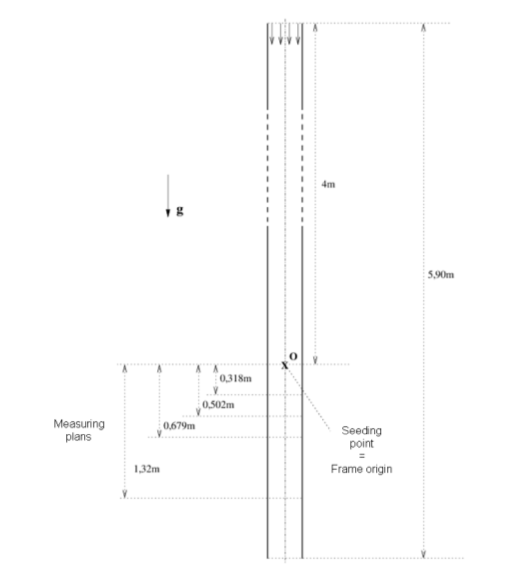
\includegraphics[width=10cm]{\IMAGES/Part2_Particle_dispersion/Schema_Arnason.png}
\caption{Schematic description of the Arnason experimental set-up \cite{Arnason}}\label{lag:Schema_Arnason}
\end{figure}

The dimensions of the pipe and the distance from the air inlet to the injection point are listed in \tablename~\ref{lag:pipe_dim} for clarity.

\begin{table}[H]
\begin{center}
\begin{tabular}{c p{4cm} c}
\Mline
\bf Pipe Internal  & \multicolumn{1}{c}{\multirow{2}{*}{\bf Pipe Length(m)}} & \bf Distance from Inlet  \\
\bf Diameter(m) & & \bf to Injection (m) \\
\hline\hline
$0.09$ & \multicolumn{1}{c}{$5.9$} & $4.0$ \\
\Mline
\end{tabular}
\caption{Arnason pipe dimensions.\label{lag:pipe_dim}}
\end{center}
\end{table}

As can be seen in \figurename~\ref{lag:Schema_Arnason}, four measuring planes were used to obtain measurements of the air flow and the glass beads.  These four planes are located downstream of the bead injection point with their positions relative to this point listed in \tablename~\ref{lag:measurement_plane}.

\begin{table}[H]
\begin{center}
\begin{tabular}{c p{6cm}}
\Mline
\bf Plane & \multicolumn{1}{c}{\bf \ \ \ \ \ Distance from injector(m) \ \ \ \ \ } \\
\hline\hline
$1$ & \multicolumn{1}{c}{$0.318$} \\  
$2$ & \multicolumn{1}{c}{$0.502$} \\ 
$3$ & \multicolumn{1}{c}{$0.679$} \\ 
$4$ & \multicolumn{1}{c}{$1.320$} \\                 
\Mline
\end{tabular}
\caption{Distance of the measuring planes downstream of the injector.\label{lag:measurement_plane}}
\end{center}
\end{table}

The flow physics are described next.



\subsection{Flow Physics}


The flow in the pipe is incompressible, fully developed, turbulent, with the air carrier phase transporting and diffusing a second phase.  Given that the second phase is dilute with respect to the carrier fluid, it is possible to assume that the glass beads are influenced by the flow of air but have no influence on the magnitude and flow direction of the carrier fluid.  This simplified modelling is known as one-way coupling.

The test rig operating conditions are described next.


\subsection{Operating Conditions}


The experimental test rig was operating with the following conditions:

\begin{itemize}
\item The maximum air velocity is of the order of 9.56m/s
\item The Reynolds number based on this maximum velocity is $50 \times 10^{3}$
\item The Reynolds number based on the mean velocity is $42\times 10^{3}$
\end{itemize}

The air temperature at inlet to the pipe is not provided in \cite{Arnason} so it is assumed to be $10^{\circ}C$.

Two sets of experiments are carried out with two different sets of glass beads and identical carrier fluid conditions.  The first set uses a bead diameter of $5\mu m$ and the second set a bead diameter of $57\mu m$.

The fluid properties are described next.


\subsection{Fluid Properties}

The fluid properties at the inlet temperature of $10^{\circ}C$ are listed in \tablename~\ref{lag:fluid_prop}.



\begin{table}[H]
\setlength\extrarowheight{5pt}
\begin{center}
\begin{tabular}{c c}
\Mline
\multirow{1}{*}{\bf $\rho (kg/m^3)$} & \multirow{1}{*}{\bf $\mu(Pa.s)$} \\
\hline\hline
\multirow{1}{*}{$1.2361$} & \multirow{1}{*}{$1.78*10^{-5}$} \\                  
\Mline
\end{tabular}
\caption{Fluid properties.\label{lag:fluid_prop}}
\end{center}
\end{table}

The properties of the glass beads are described next.



\subsection{Glass Beads} \label{lag:glass_beads}

The properties of the $5\mu m$ glass beads are listed in \tablename~\ref{lag:bead_prop}.

\begin{table}[H]
\setlength\extrarowheight{5pt}
\begin{center}
\begin{tabular}{c p{6cm} c}
\Mline
\multirow{1}{*}{\bf Mean diameter} & \multicolumn{1}{c}{\multirow{1}{*}{\bf \ \ \ \ Diameter Deviation \ \ \ \ }} & \multirow{1}{*}{\bf Density}\\
\multirow{1}{*}{\bf $d_p^{\mu}(\mu m)$} & \multicolumn{1}{c}{\multirow{1}{*}{\bf $\sigma_p(\mu m)$}} & \multirow{1}{*}{$\rho (kg/m^3)$} \\
\hline\hline
\multirow{1}{*}{$5.0$} & \multicolumn{1}{c}{\multirow{1}{*}{$1.0$}} & \multirow{1}{*}{$2475$} \\                  
\Mline
\end{tabular}
\caption{Glass bead properties.\label{lag:bead_prop}}
\end{center}
\end{table}

The particle diameter $d_p$ is calculated from the mean diameter and the deviation by $d_p=d_p^{\mu}+\varepsilon*\sigma_p$, where $\varepsilon$ is a random variable which follows a normal law.

The boundary conditions are discussed next.

\subsection{Boundary Conditions}

Three carrier fluid boundary conditions are used in this study: inlet, outlet and wall.  For the particles, the only boundary condition used is wall. \figurename~\ref{lag:Location_BC} illustrates the location of these boundary conditions and the flow direction (blue arrows).

\begin{figure}[H]
\centering
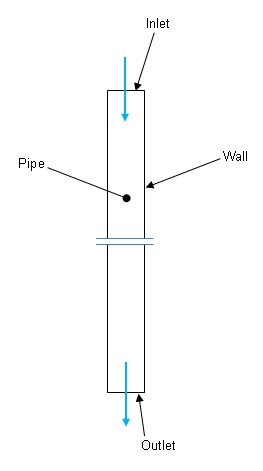
\includegraphics[width=5cm]{\IMAGES/Part2_Particle_dispersion/location_BC_crop.png}
\caption{Location of the boundary conditions.}\label{lag:Location_BC}
\end{figure}

\tablename~\ref{lag:bc_air_part} lists the various boundary values applied for the carrier fluid (air) and the particles.

\begin{table}[H]
\begin{center}
\begin{tabular}{c | c p{3cm} c}
\Mline
\bf Phase & \multicolumn{3}{c}{\bf \ \ \ \ \ \ \ \ \ \ \ \ \ Boundary Conditions and Values}   \\
 & \bf Inlet & \multicolumn{1}{c}{\bf Outlet} & \bf Wall \\
\hline\hline
\multirow{4}{*}{\bf Air} & \multicolumn{1}{l}{$u=0$} & \multicolumn{1}{c}{\multirow{4}{*}{Standard}}& \multirow{4}{*}{Wall} \\
 &\multicolumn{1}{l}{$v=0$}& & \\
 &$w=-V_{max}(1.0-\dfrac{0.4 \times r^2}{0.002025}) $& & \\
 &\multicolumn{1}{l}{$D_h=0.09m$}& & \\ 
\bf Particles & - & \multicolumn{1}{c}{-} & Rebound \\                  
\Mline
\end{tabular}
\caption{Boundary conditions and values for the air and the particles.\label{lag:bc_air_part}}
\end{center}
\end{table}

The inlet boundary condition corresponds to a Reynolds number of 42000 based on the mean velocity which itself corresponds to a mass flow rate of 0.06291kg/s.  A correction factor of 1.0488 is used to maintain the Reynolds number.

In the Arnason experiment, the particles are injected along the centre line of the pipe at the reference point.  Since the particle injection velocity is not given in \cite{Arnason}, in this tutorial we assume that it is equal to the local fluid velocity.

Also, the results presented in \cite{Arnason} do not stipulate the number of particles injected, the results only give statistical data.  For the simulations in this tutorial, 1000 particles are injected per time step in order to have a sufficient number of particles to post process.

Lastly, in the CFD model the turbulence at the inlet boundary is calculated directly by \CS using the hydraulic diameter, $D_h$, specified.

\subsection{One-Way Coupling CFD Modelling}\label{lag:one_way}

The one-way coupling simulation of the two-phase flow of the air and the glass beads is broken into two steps.  First, the flow of air alone is simulated.  This will be used as the background flow on which the particles are injected.  Then, in the second step, the flow of the particles on top of this air flow field is calculated.

\subsection{Creating \CS Study}\label{lag:create_CS_struct}

A \CS study called \textit{ARNASON} and a first case are created. This first case will be set up as a single-phase calculation. Call it \textit{RANS\_rij\_SSG}.

The study and the case are created using the procedure described in Part I of tutorial 1 \cite{ShearDriven_Tuto}.  Start \salome\_CFD, select the CFDStudy module, and go through all the steps detailed in \cite{ShearDriven_Tuto} to:

\begin{itemize}
\item Create the CFD study/case structure with the CFDStudy module
\item Save the new file as 'ARNASON'
\end{itemize}


\begin{figure}[h]
	\begin{minipage}[c]{.46\linewidth}
		\centering
		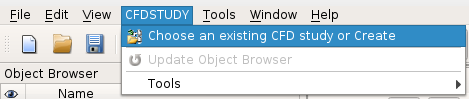
\includegraphics[scale = 0.6]{\IMAGES/create_cfd_study_salome8.png}
		\caption{\textit{Create a CFD study}}
		\label{lag:create_cfd.png}
	\end{minipage}
	\hfill%
	\begin{minipage}[c]{.40\linewidth}
		\centering
		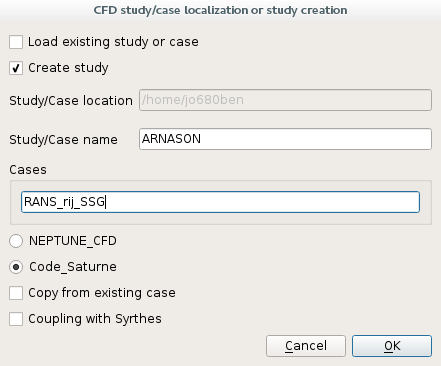
\includegraphics[scale = 0.5]{\IMAGES/cfd_study_salome8.png}
		\caption{\textit{CFD study localization or creation}}
		\label{lag:cfd_study}
	\end{minipage}
\end{figure}


In the end, you should end up with the directory structure (\figurename~\ref{lag:arbre_cfd_study}) shown in the Object Browser tab, displaying the study and the first case.

\begin{figure}[H]
	\centering
	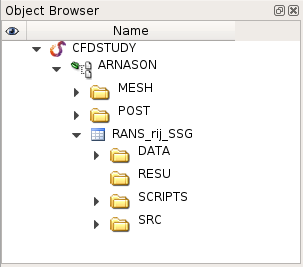
\includegraphics[scale=0.7]{\IMAGES/arbre2_salome8.png}
	\caption{\textit{ARNASON} Study, \textit{RANS\_rij\_SSG} case File Structure}\label{lag:arbre_cfd_study}
\end{figure} 

The case is then ready to be set up.

\section{Creating the Computational Domain}
%
\subsection{What you will Learn (Geom and Smesh)}
In this part, you will learn how to create the computational domain using the \geom and \smesh modules of \salome. Thanks to primitives available in \geom, creating the CAD will be easy and the work will essentially be in \smesh.
%
\subsection{Creating the CAD}
%
Once the files structure is created by following the step in \ref{lag:create_CS_struct}, move to the \geom module in \salome. We want to create two cylinders which will subsequently define two zones in the flow domain, upstream and downstream of the injection plane, respectively. The reason for creating two cylinders is that the mesh upstream of the injection point will be coarser than that downstream of it.  This will not have an impact on solution accuracy but will reduce the overall computational time. In the present part, a disk is created. In the following parts, it will be meshed and finally extruded to generate the two cylinders.

Create a Divided Disk by selecting \menu{New Entity > Blocks > Divided Disk}. This represents the inlet boundary:
%
\begin{itemize}
	\item \textbf{name:} inlet\_disk 
	\item  \textbf{Radius:} 0.045
	\item \textbf{Orientation:} OXY
	\item \textbf{Division pattern:} Hexagon
\end{itemize} 
%
\begin{figure}[hbtp]
	\centering
	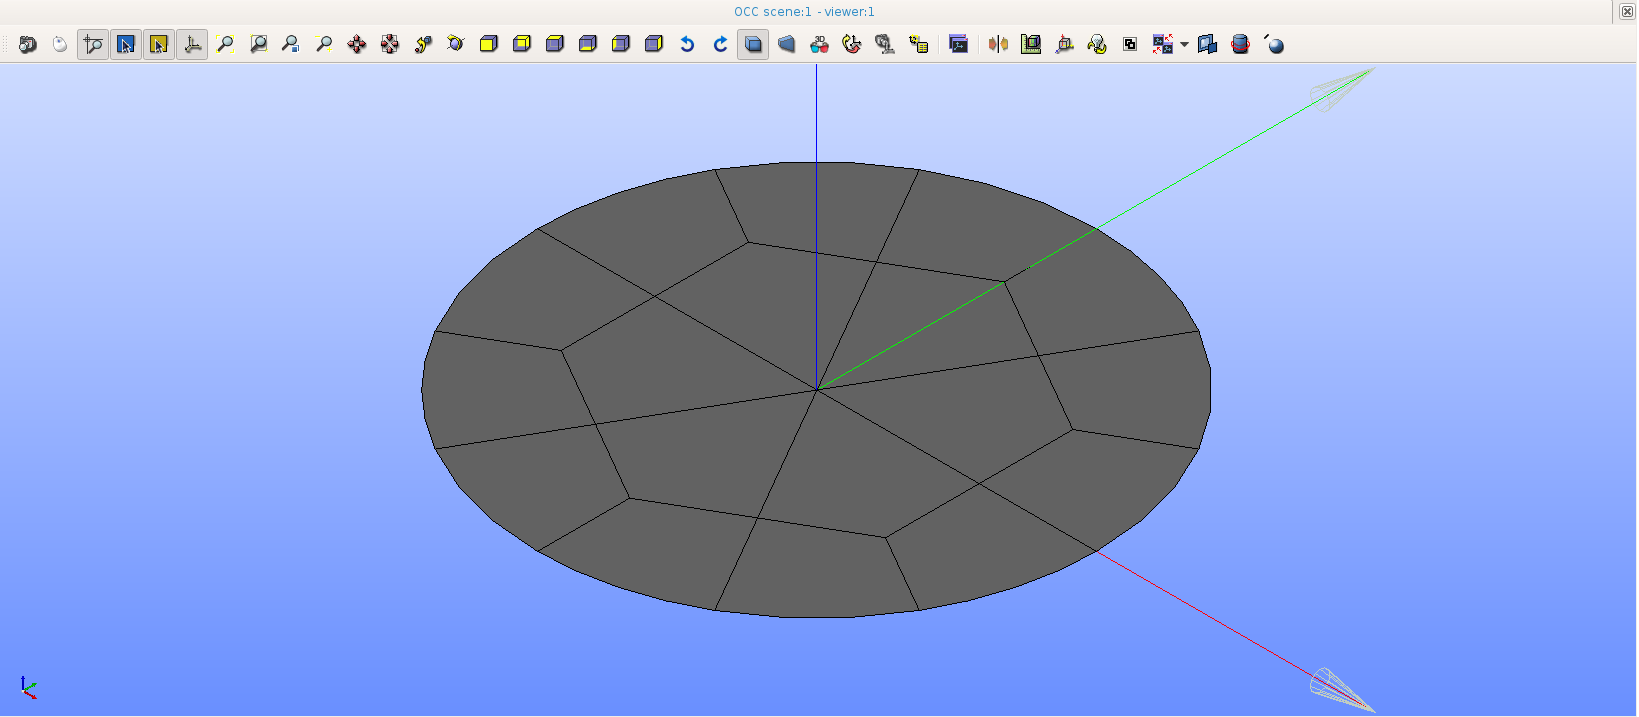
\includegraphics[width=0.8\textwidth]{\IMAGES/scdcylinder.png}
	\caption{Divided disk}
	\label{lag:scd_cylinder}
\end{figure}
%

Finally, create the two following points:
\begin{itemize}
	\item \textbf{name:} z\_4.0
	\item  \textbf{Coordinates} x: 0; y: 0, z: 4.0
\end{itemize} 
%
\begin{itemize}
	\item \textbf{name:} z\_5.9
	\item  \textbf{Coordinates} x: 0; y: 0, z: 5.9
\end{itemize} 
%
and the two following lines:
\begin{itemize}
	\item \textbf{name:} 0\_to\_4.0
	\item \textbf{Point 1:} O (origin, clic on O in Object Browser)
	\item \textbf{Point 2:} z\_4.0
\end{itemize} 
%
\begin{itemize}
	\item \textbf{name:} 4.0\_to\_5.9
	\item \textbf{Point 1:} z\_4.0 
	\item \textbf{Point 2:} z\_5.9
\end{itemize} 
%
\subsection{Creating Groups on \geom}
%
The next step is
to create some groups that will be used as boundary conditions by the numerical model.

Right click on inlet\_disk and select \textbf{Create Group}.
Select the edges composing the border of the disk and add them to the group (\figurename~\ref{lag:wall_group}). It will be our boundary condition "wall".
%
\begin{itemize}
	\item \textbf{Shape Type:} edges
	\item \textbf{Group Name:} wall
	\item \textbf{Main Shape:} inlet\_disk
	\item \textbf{Main Shape Selection restriction}: No restriction
\end{itemize}
%
\begin{figure}[H]
	\centering
	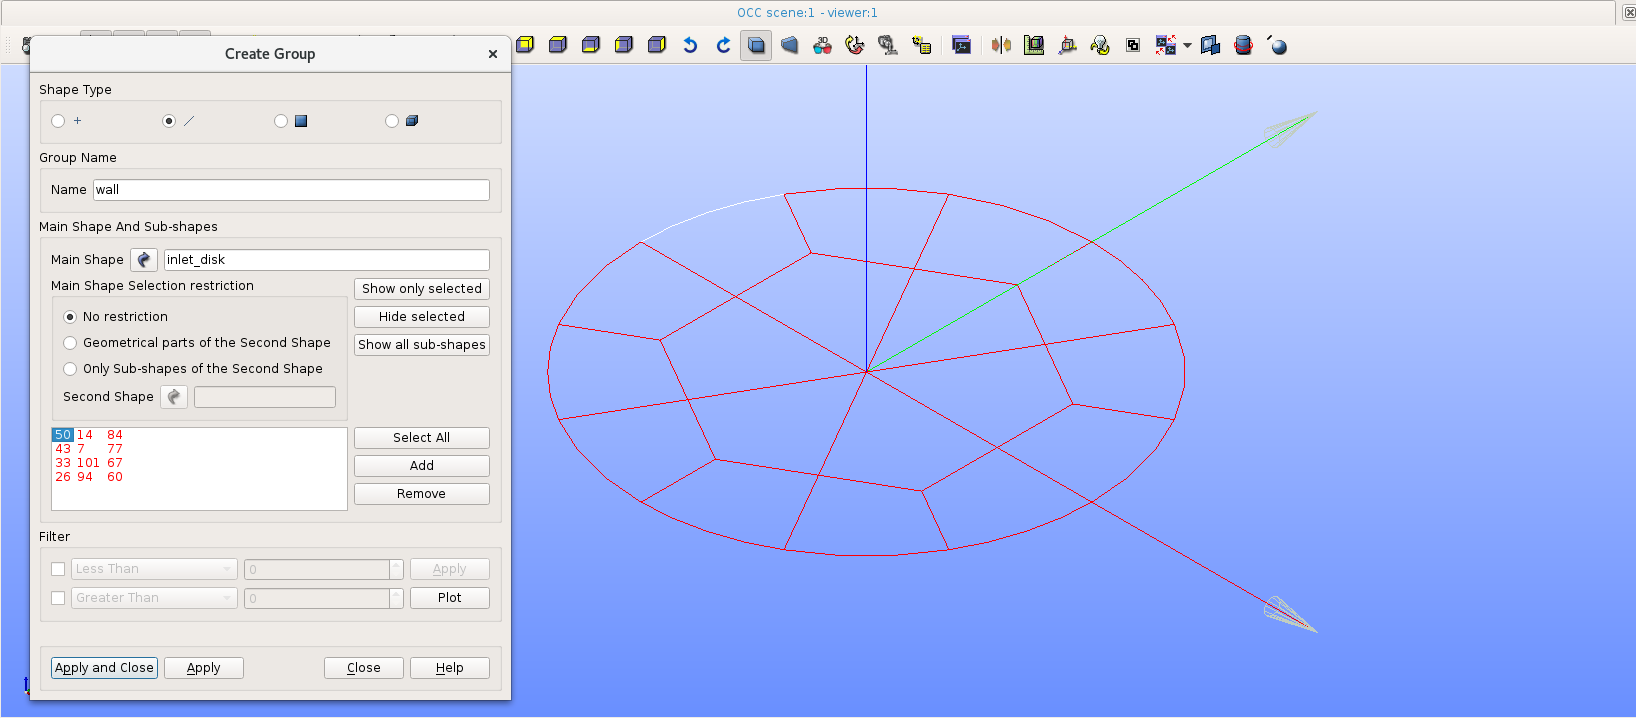
\includegraphics[width =\linewidth]{\IMAGES/wall_point.png}
	\caption{Creation of the group ``wall''}
	\label{lag:wall_group}
\end{figure}
%
\clearpage
%
\subsection{Meshing}
%
Move to the module 'Mesh' (\smesh) of \salome. Select inlet\_disk in the object browser and \menu{Mesh > Create Mesh}.
%
\begin{itemize}
	\item \textbf{Name:} inlet\_mesh
	\item \textbf{Geometry:} inlet\_disk
	\item \textbf{Mesh type:} Any
	\item \menu{2D > Algorithm} ``Quadrangle: Mapping''
	\item \menu{1D > Algorithm} ``Wire Discretisation''
	\item \menu{1D > Hypothesis} ``Number of segments'' with arguments 4 and ``Equidistant distribution''
\end{itemize}
%
\begin{figure}[H]
	\centering
	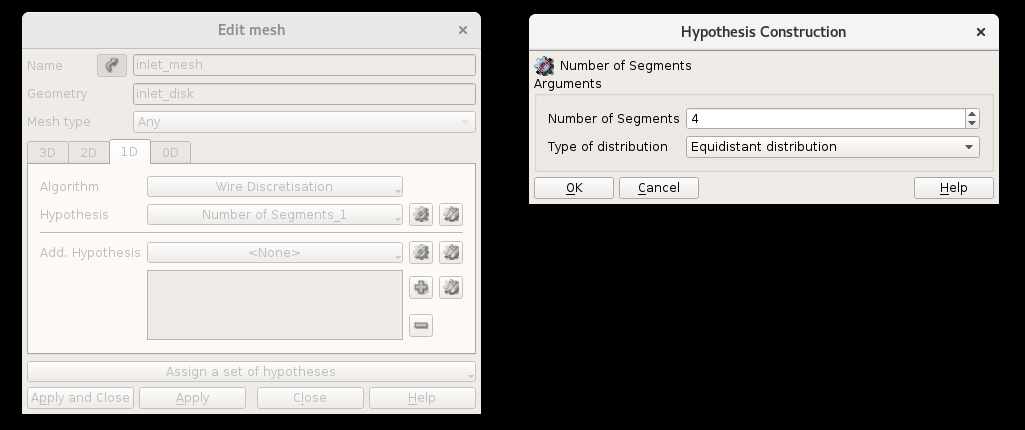
\includegraphics[width =\textwidth]{\IMAGES/3d_mesh.png}
	\caption{Create Mesh}
	\label{lag:mesh_01}
\end{figure}
%
Apply.

In order to prepare the extrusion of the inlet disk, the best way is to mesh two lines following the z-axis and extrude the cylinder along these two lines. The refinement of the lines mesh will be the final refinement of the cylinder in the z-direction. Refinement are set as follows:

Mesh of the first section: 0\_to\_4.0 line
%
\begin{itemize}
	\item \textbf{Name:} 0\_to\_4.0\_mesh
	\item \textbf{Geometry:} 0\_to\_4.0
	\item \textbf{Mesh type:} Any
	\item \menu{1D > Algorithm:} ``Wire Discretisation''
	\item \menu{1D > Hypothesis > Number of segments}: 100 and ``Scale distribution'' with a scale factor of 0.045
\end{itemize}
%
Apply.

Mesh of the second section:
%
\begin{itemize}
	\item \textbf{Name:} 4.0\_to\_5.9\_mesh
	\item \textbf{Geometry:} 4.0\_to\_5.9
	\item \textbf{Mesh type:} Any
	\item \menu{1D > Algorithm:} ``Wire Discretisation''
	\item \menu{1D > Hypothesis > Number of segments} 422 and ``Equidistant distribution''
\end{itemize}
%
Apply.

Then create a mesh group lying on the ``wall'' group created in \geom, by right clicking in the object browser on inlet\_mesh
and selecting \menu{Create Groups from Geometry}. Add the geometry group ``wall'' to the Elements list (\figurename~\ref{lag:ext_wall}).
%
\begin{figure}[H]
	\centering
	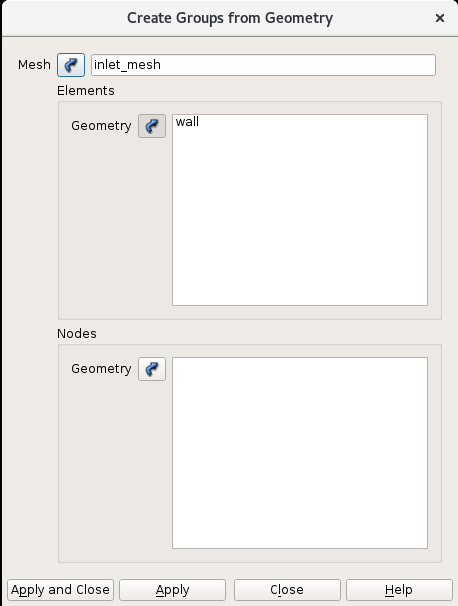
\includegraphics[width = 0.6\textwidth]{\IMAGES/ext_wall.png}
	\caption{Create Groups from Geometry}
	\label{lag:ext_wall}
\end{figure}
%
Compute all meshes (inlet\_mesh, 0\_to\_4.0\_mesh and 4.0\_to\_5.9\_mesh) by right clicking on each mesh and selecting \menu{Compute}.
%
\subsection{Creating Groups in \smesh}
%
Right click on inlet\_mesh and \textbf{Create Group}
%
\begin{itemize}
	\item \textbf{Mesh:} inlet\_mesh
	\item \textbf{Elements Type:} Face
	\item \textbf{Name:} inlet
	\item \textbf{Content:} Select all
\end{itemize}
%
Apply and close.

Now the disk is well discretized and just needs to be extruded along each z-section.

For the first section, select \menu{Modification > Extrusion along a path} and fill the pop-up window as follows:
%
\begin{figure}[H]
	\centering
	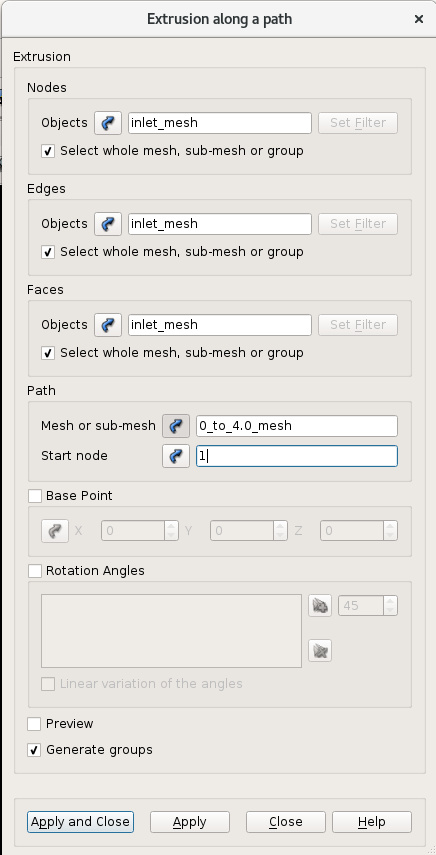
\includegraphics[scale = 0.5]{\IMAGES/extr_1.png}
	\caption{Extrusion along 0\_to\_4.0\_mesh}
	\label{lag:extr_1}
\end{figure}
%
Apply and close.

In Groups of Faces, rename inlet\_top as injection\_plane.

We then need to create a group of cells in which particles will be injected at each iteration of the lagrangian computation.
For this, right click on inlet\_mesh, and select \menu{Create group}. Fill the pop-up window with following settings:
%
\begin{itemize}
	\item \textbf{Mesh:} inlet\_mesh
	\item \textbf{Elements Type:} Volume
	\item \textbf{Name:} injection
	\item \textbf{Group type:} Standalone group
	\item \textbf{Enable manual edition:} toggled
\end{itemize}
%
And select manually the cells around the pipe axis at the injection plane as shown on \figurename~\ref{lag:injection_volume}:
%
\begin{figure}[H]
	\centering
	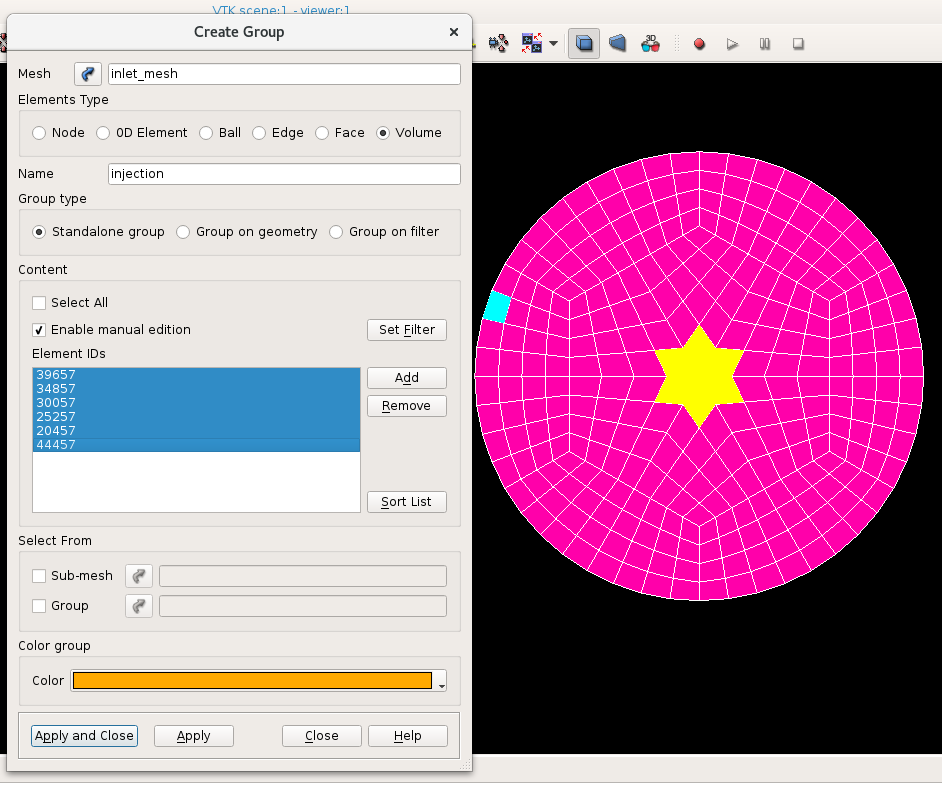
\includegraphics[width=0.8\textwidth]{\IMAGES/injection_group_creation.png}
	\caption{Creation of the injection group}
	\label{lag:injection_volume}
\end{figure}
%
Finally, select the group injection\_plane, created above, and extrude it along 4.0\_to\_5.9.mesh (\figurename~\ref{lag:extr_2}):
%
\begin{figure}[H]
	\centering
	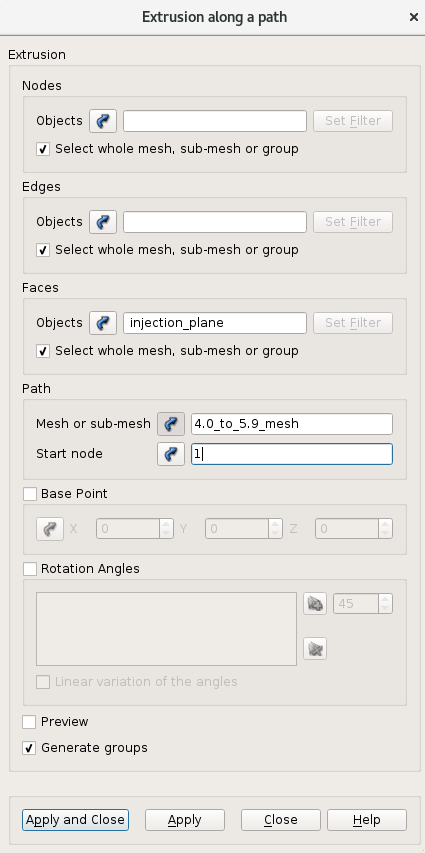
\includegraphics[scale = 0.5]{\IMAGES/extr_2.png}
	\caption{Extrusion along 4.0\_to\_5.9\_mesh}
	\label{lag:extr_2}
\end{figure}
%

Remove all groups of Groups of Edges. In Groups of Faces, select wall\_extruded and wall\_top\_extruded (with \keys{Ctrl}) , click on \menu{Mesh > Union groups} and name it wall.
Apply and close, then remove wall\_top\_extruded and wall\_extruded.
Rename also injection\_plane\_top as outlet. Finally, remove all groups of Groups of Volumes, except, of course, injection. You can also change the groups colors to be able to distinguish them clearly.
%
\clearpage
%
You should get a final mesh as shown on \figurename~\ref{lag:final}.
%
\begin{figure}[H]
	\centering
	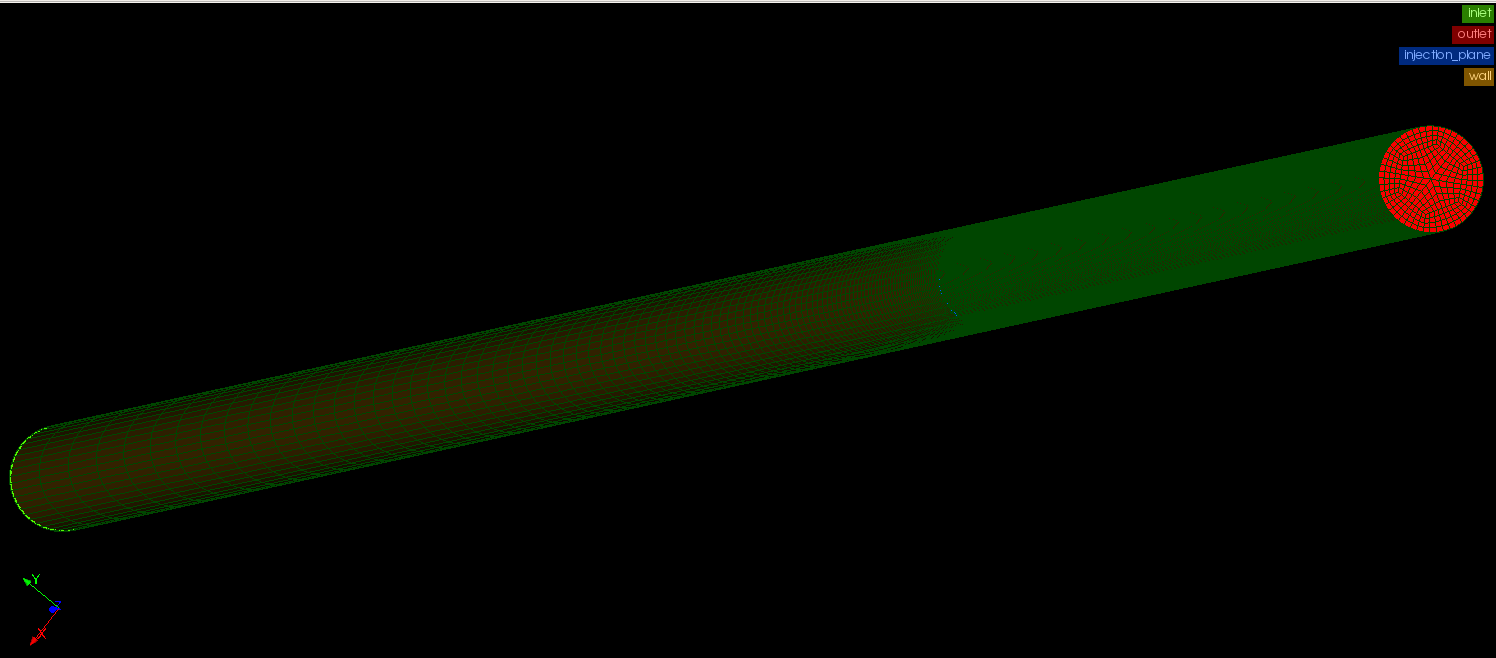
\includegraphics[width = \linewidth]{\IMAGES/final_pipe_mesh.png}
	\caption{volume mesh}
	\label{lag:final}
\end{figure}
%

Two last transformations will be applied to the mesh.

Select \menu{Modification > transformation > Symmetry}.
Toggle \keys{Select whole mesh, sub-mesh or group} and select inlet\_mesh as Name in Arguments.
Apply and close.

Select \menu{Modification > transformation > Translation} and fill the pop-up window as follows (\figurename~\ref{lag:translate}):
%
\begin{figure}[H]
	\centering
	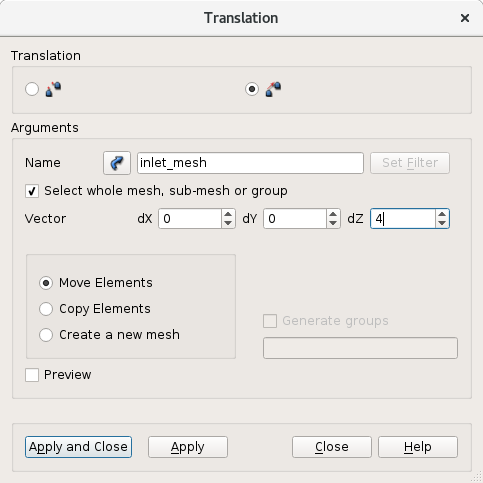
\includegraphics[width=0.7\textwidth]{\IMAGES/translate_mesh.png}
	\caption{Translation of mesh}
	\label{lag:translate}
\end{figure}
%
Apply and Close.

The generation of the computational domain is now completed. Save the \salome file and export the mesh file in ‘.med’ format by selecting from the main menu: \menu{File > Export > MED file}. For the file name, choose ‘Mesh\_ARNASON’; the ‘.med’ extension is automatically added.  You are now ready to move to the CFDStudy module in order to set up the CFD simulation.

\section{Single-Phase RANS Computation}
%
\subsection{What you Will Learn}
%
In this part of the tutorial you will learn how to set-up, run, and post-process the results of a steady-state single phase RANS calculation for the Arnason pipe generated in the previous Section, using the CFDStudy module in \salome. You will also learn how to integrate user defined functions into a \CS calculation. The user defined functions will be used to specify the inlet boundary conditions. Probes will also be set in the computational domain and used in the analysis to verify that steady-state, converged results are obtained.
%
\subsection{Setting up the CFD Simulation}
%
The CFD case is set-up and run from the CFDStudy module (Section \ref{lag:create_CS_struct}). 

In the CFDStudy module, launch the CFDStudy GUI and verify that the case directory structure has been correctly recognised by clicking on the \textbf{Identity and Paths} folder in the tree menu.  If the case directory is correct you can continue.  If not, you will need to set the correct directory.  Then, save the CFD data file. By default, its name will be setup.xml.

You can now proceed with setting up the case, following the top-down order of the folders in the left-hand column, starting with the mesh.

\subsubsection{Selecting the Volume Mesh}

Go to the {\color{eblue} \bf Mesh} section  and, in the \menu{List of meshes} add the mesh ‘Mesh\_ARNASON.med’. This is done by clicking on the \keys{$+$} icon in the panel and selecting the appropriate mesh in the MESH directory, as shown in \figurename~\ref{lag:import_mesh}.  No further input is necessary for the volume mesh.
%
\begin{figure}[H]
\centering
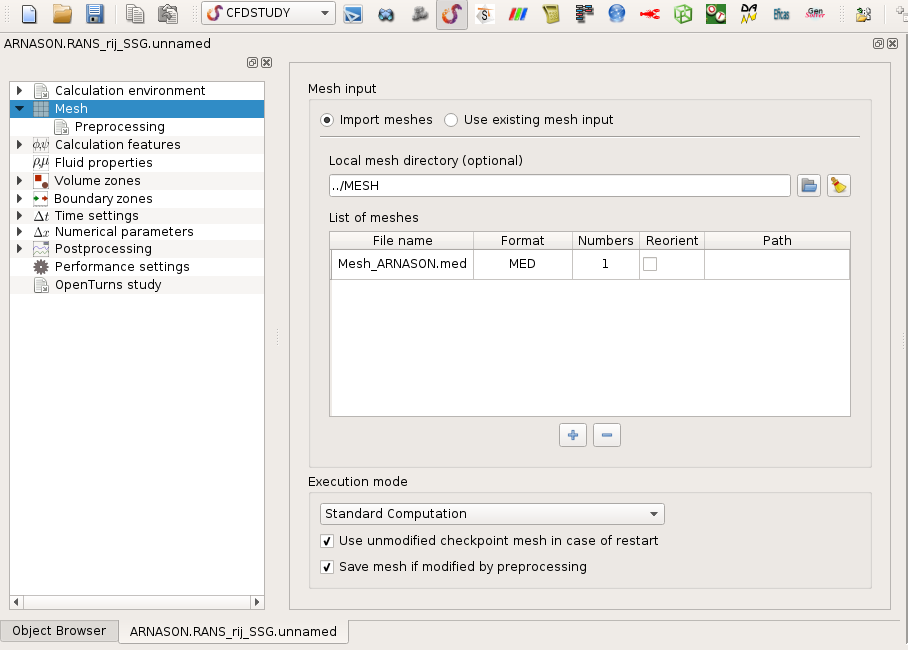
\includegraphics[width=0.6\textwidth]{\IMAGES/Part4_RANS/import_mesh.png}
\caption{Importing the mesh.}\label{lag:import_mesh}
\end{figure}
%

\subsubsection{Calculation features}

In the \textbf{Calculation features} section, leave all options to their default values, i.e. only \textbf{Standard Eulerian single phase} is selected.

In the \textbf{Turbulence models} sub-section, change the \textit{Turbulence model} to \textit{Rij-epsilon SSG}.  In the \textbf{Advanced Options} menu, ensure that the wall function type is set to ‘Two scales model’ and that ‘Gravity terms in the turbulence equations’ is selected.

In the \textbf{Body forces} sub-section, set the acceleration of gravity by entering the value ‘$-9.81 m/s^2$’ for its component in the vertical (Z) direction in the ‘Gravity’ panel.

Now you can go to the \textbf{Fluid Properties} section.

\subsubsection{Physical Properties}

Given that the flow field is incompressible, the physical properties of the fluid are constant for a constant fluid temperature of \textbf{$10^{\circ}C$}.  Specify the value of each fluid property as shown in \figurename~\ref{lag:fluid_prop_gui}.
%
\begin{figure}[H]
\centering
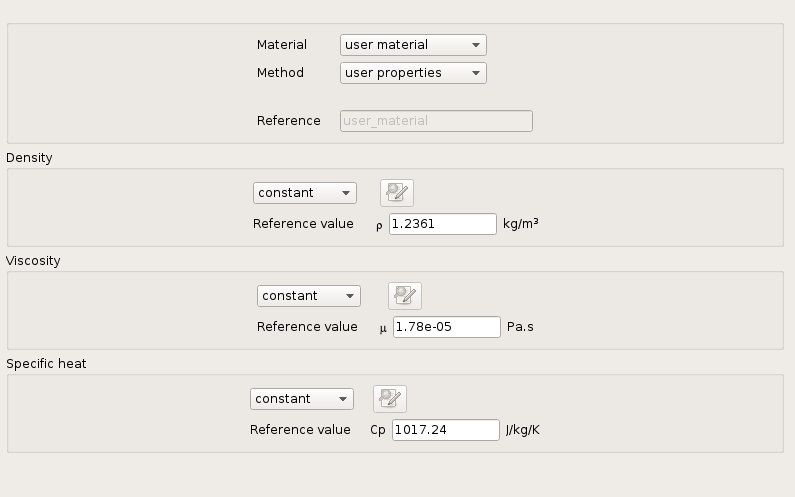
\includegraphics[width=0.6\textwidth]{\IMAGES/Part4_RANS/Fluid_properties.png}
\caption{Specifying the fluid properties.}\label{lag:fluid_prop_gui}
\end{figure}
%


No other settings are required in this folder.  You can now move to the \textbf{Initialization} under the \textbf{Volume zones} section.

\subsubsection{Initialization}

The initial values for the velocity are defined in the ‘Initialization’ tab. The flow is initially stagnant by default.

No other settings are required in this folder.  You can now move to the ‘Boundary zones’ section.

\subsubsection{Boundary zones}\label{lag:inlet_outlet_BCs}

Three boundary conditions are used in this study: inlet, wall and outlet.  These conditions are listed in \tablename~\ref{lag:bc_air_part}.   The inlet boundary condition will be defined in the ‘cs\_user\_boundary\_condition’ subroutine so it does not need to be generated here (see \ref{lag:code_inlet}).

First, create the 'wall' and 'outlet' boundary regions by selecting the wall and outlet group in \salome object browser and by clicking on \keys{Add from Salome} (\figurename~\ref{lag:def_bc}).  Finally, change the type ('Nature') of the boundary to ‘outlet’ for the outlet boundary but leave the type of the wall boundary condition as ‘wall’.
%
\begin{figure}[H]
\centering
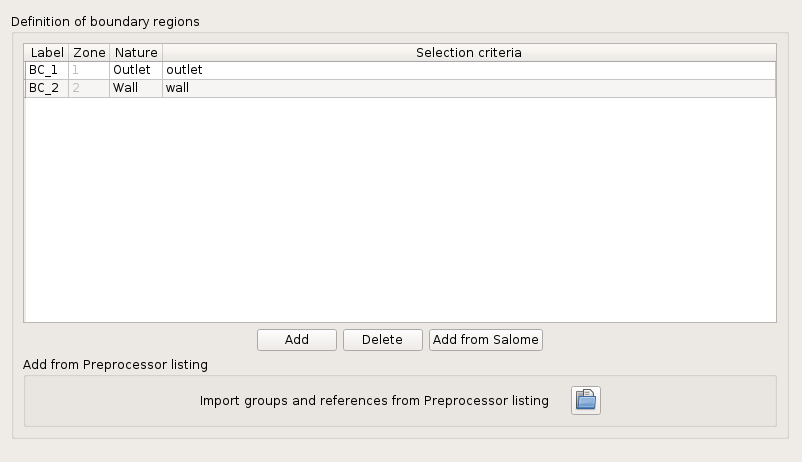
\includegraphics[width=0.6\textwidth]{\IMAGES/Part4_RANS/def_bc.png}
\caption{Defining the boundary conditions.}\label{lag:def_bc}
\end{figure}
%
Having defined their type, the values to apply at each boundary could now be specified.  However, as the default values are used in this tutorial, no further specification is necessary.  To check the default values, select the ‘Boundary conditions’ sub-folder and click on the boundary of interest.

No other settings are required in this folder. You can now go to the ‘Numerical parameters’ folder.

\subsubsection{Numerical Parameters}

In the \keys{Equation parameters} sub-folder, the \keys{Solver} panel shows that pressure, velocity, turbulent kinetic energy and turbulent kinetic energy dissipation are solved for. In order to decrease overall computation time, it is possible to decrease the solver precision by setting the convergence criterium to $10^{-5}$ for each variable, except for pressure, without having an impact on solution quality.

In the \keys{Time step} panel, set the time step to 0.01s and the number of iterations to 850.  For this tutorial, this number of iterations is sufficient to reach a steady-state flow solution.

\subsubsection{Calculation Control}

In the \keys{Calculation control} folder, select the \keys{Output control} sub-folder and go into the \keys{Monitoring Points} panel.  Click on the \keys{$+$} icon to add a probe, then enter the coordinate of the probe.  Repeat this procedure for the probes of your choice.  Monitoring probes can be useful to check the convergence of the simulation and it is recommended that monitoring points are specified along the axis of the pipe after the particle injection point.  The monitoring points used for this tutorial are shown in \figurename~\ref{lag:monitoring}. Select the \keys{csv} format in order to be able to open the output files in \paravis.
%
\begin{figure}[H]
\centering
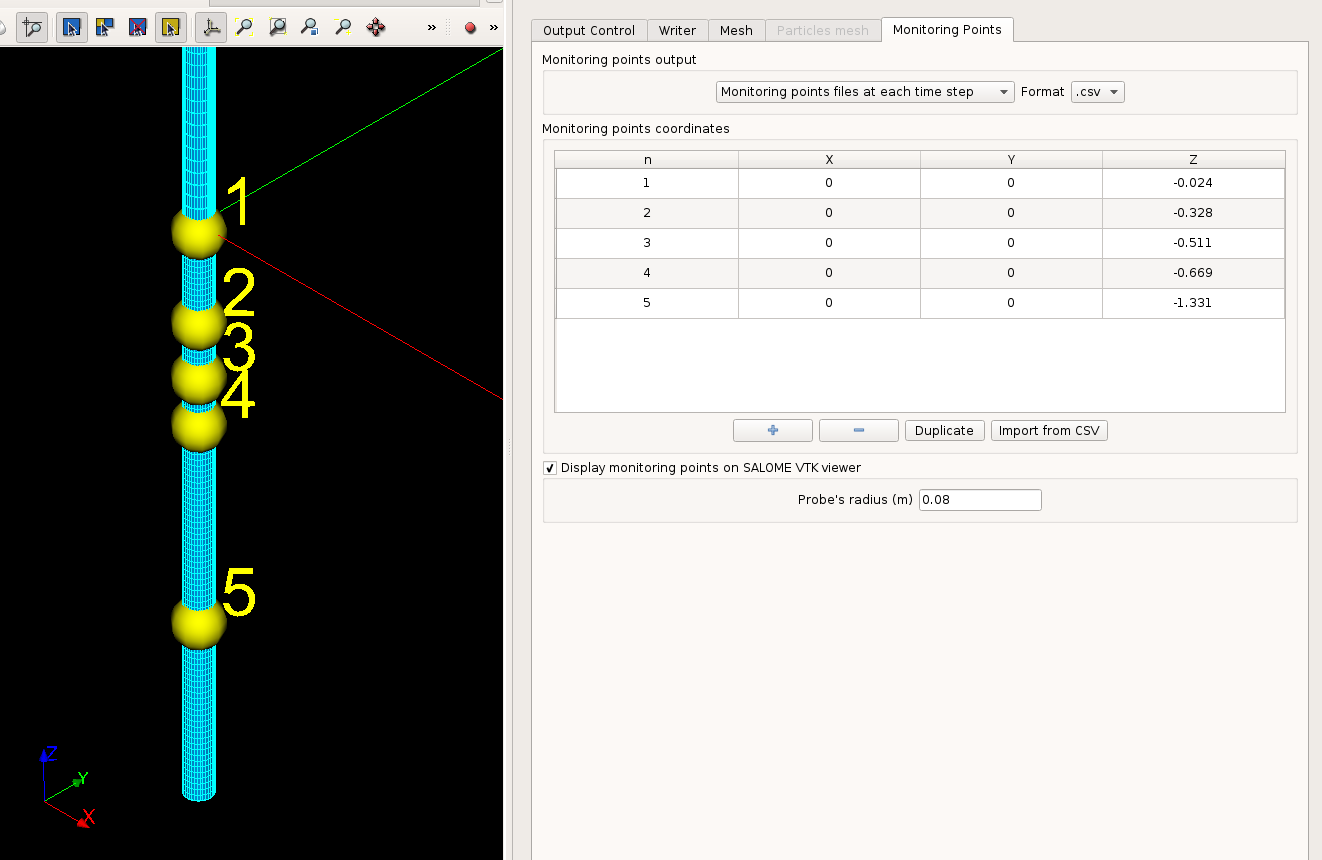
\includegraphics[width=\textwidth]{\IMAGES/Part4_RANS/monitoring_points_v2.png}
\caption{Monitoring points.}\label{lag:monitoring}
\end{figure}
%
The \CS calculation is now fully specified from the standpoint of the GUI and the \CS case 'xml' file should be saved.  However, prior to running the simulation, the inlet boundary condition still needs to be specified.  A parabolic law defining the $V_z$ velocity component needs to be coded in the ‘cs\_user\_boundary\_conditions.f90’ subroutine.  This step is described next.

\subsubsection{Programming the Inlet Boundary Condition}\label{lag:code_inlet}

To begin with, copy the sample file ‘cs\_user\_boundary\_conditions-base.f90’ from the tutorial $/../ARNASON/\\RANS\_rij\_SSG/SRC/EXAMPLES$ directory to your SRC directory.  This is done in order to create a local copy which you will be able to customise and which will be automatically recompiled and linked to the ‘cs\_solver’ executable at run time.

Once copied, open your local version of the file by a right-click on it in the object browser or by using the text editor of your choice.  This subroutine contains several examples of different boundary conditions that can be used by \CS.  In this tutorial, you will customise ‘Example 1’ with your own implementation of the $V_z$ velocity as a function of radius (Eq. \ref{lag:bc_air_part}).  To keep your code clean, you may remove all the other examples from the file.  The customised code is available with this tutorial and is already commented.  Here we describe the main parts of this user coding and the logic behind them.
%
\begin{enumerate}
\item Declare your own local variables at the top of the subroutine, either as double precision real values or integer values
\item Initialise your own local variables
\item Use the subroutine ‘getfbr’ to select the faces attached to the ‘inlet’ boundary condition
\item Cycling through the boundary faces.
\begin{enumerate}
\item Apply the type ‘entre’ to all boundary faces
\item Calculate the $V_z$ velocity component and the turbulence based on the hydraulic diameter
\end{enumerate}
\end{enumerate}
%
\subsection{Running and Analysing the Simulation}

\subsubsection{Running the Simulation}

To launch the simulation, click on the {\color{eblue} \bf Run or submit solver} button as shown below:

\begin{figure}[H] 
\centering
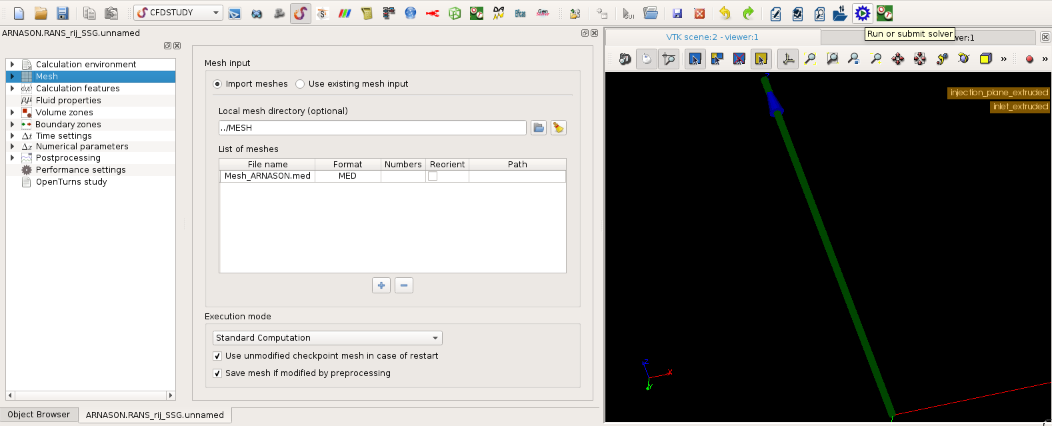
\includegraphics[width=\textwidth]{\IMAGES/Part4_RANS/run_submit_solver.png} 
\caption{Run}
\label{lag:cap1_run}
\end{figure}

A window will open where you can specify the run options.

All options except the number of processes are let to their default values:
%
\begin{itemize}
\item ‘runcase’ for the ‘Script file’
\item ‘1’ for the number of threads per process
\item build type to '[default]'.
\end{itemize}
%
You may increase the ‘Number of processes’, depending on the number of cores available on your machine in order to run the simulation in parallel.
With the provided mesh (150336 cells), 4 processes would lead to a nearly optimal speed up. To give a rough idea, this calculation can take slightly less than half an hour if run on only one process.

To run \CS, press the ‘Save case and run calculation’ button.  The pop-up panel for the run opens, listing in real time the different stages of the calculation, from user-subroutines compilation to saving the results.

\subsubsection{Checking Calculation Convergence}

Wait for the calculations to complete and open the ‘listing’ file in your "ARNASON/RANS\_rij\_SSG/\\RESU/DateOfRunTimeOfRun/" directory.  Verify that the residuals listed under 'time residual' in the ‘Information on Convergence’ table have dropped several orders of magnitude for all variables (pressure, velocity and temperature), showing that the calculations have fully converged to a steady-state solution (\figurename~\ref{lag:cap1_iter},~\ref{lag:cap2_iter}).
%
\begin{figure}[H]
\scriptsize{
\begin{lstlisting}
   ** INFORMATION ON CONVERGENCE
      --------------------------
----------------------------------------------------------------------------
   Variable     Rhs norm      N_iter  Norm. residual   Drift   Time residual
----------------------------------------------------------------------------
c  Velocity     0.19438E-03       2   0.94359E-04   0.63501E+04 0.10000E+03 
c  Velocity[X]                                      0.10213E-01 
c  Velocity[Y]                                      0.10213E-01 
c  Velocity[Z]                                      0.63501E+04 
c  Pressure     0.38502E-02      42   0.70117E-02   0.99811E+00 0.10000E+03 
c  Rij          0.30302E-02      47   0.16926E-01   0.11918E-01 0.98830E+02 
c  Rij[XX]                                          0.39706E-02 
c  Rij[YY]                                          0.39706E-02 
c  Rij[ZZ]                                          0.39762E-02 
c  Rij[XY]                                          0.82075E-65 
c  Rij[YZ]                                          0.43962E-36 
c  Rij[XZ]                                          0.42288E-36 
c  epsilon      0.94803E-01      51   0.62111E-01   0.13189E+03 0.10000E+03 
----------------------------------------------------------------------------
\end{lstlisting}}
\caption{Information on convergence in listing file at first iteration}\label{lag:cap1_iter}
\end{figure}
%
\begin{figure}[H]
\scriptsize{
\begin{lstlisting}
   ** INFORMATION ON CONVERGENCE
      --------------------------
----------------------------------------------------------------------------
   Variable     Rhs norm      N_iter  Norm. residual   Drift   Time residual
----------------------------------------------------------------------------
c  Velocity     0.21440E+00       1   0.11313E-02   0.29963E-03 0.21465E-01 
c  Velocity[X]                                      0.41963E-05 
c  Velocity[Y]                                      0.41665E-05 
c  Velocity[Z]                                      0.29126E-03 
c  Pressure     0.13227E-04      13   0.72886E-04   0.23426E-01 0.19810E-02 
c  Rij          0.18154E+00       1   0.59522E-05   0.21129E-06 0.80776E-02 
c  Rij[XX]                                          0.10648E-07 
c  Rij[YY]                                          0.10509E-07 
c  Rij[ZZ]                                          0.13732E-06 
c  Rij[XY]                                          0.35421E-08 
c  Rij[YZ]                                          0.23857E-07 
c  Rij[XZ]                                          0.25411E-07 
c  epsilon      0.56982E+01       2   0.70640E-05   0.13186E-01 0.26060E-01 
----------------------------------------------------------------------------
\end{lstlisting}}
\caption{Information on convergence in listing file at first iteration}\label{lag:cap2_iter}
\end{figure}
%
Further, check if the flow values are well-established and that the flow has reached a steady-state by plotting the values of velocity at the probes locations. You can use \salome module \paravis for this purpose.
%
\begin{figure}[H] 
\centering
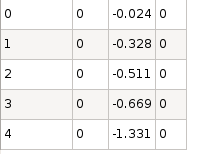
\includegraphics[width=0.3\textwidth]{\IMAGES/Part4_RANS/monitoring.png} 
\caption{Monitoring points coordinates}
\label{lag:cap1_monit}
\end{figure}
%
\figurename~\ref{lag:cap2_monit} presents the evolution of the velocity at the five monitoring points placed along the pipe axis at the z coordinates -0.024, -0.328, -0.511, -0.669 and -1.331m. This figure indicates that, after an intial transient during which the flow develops from the initial solution, the flow is well established and steady within 850 iterations. \figurename~\ref{lag:axial_velocity} shows a picture of the magnitude of the velocity at the outlet of the pipe.  
%
\begin{figure}[H]
\centering
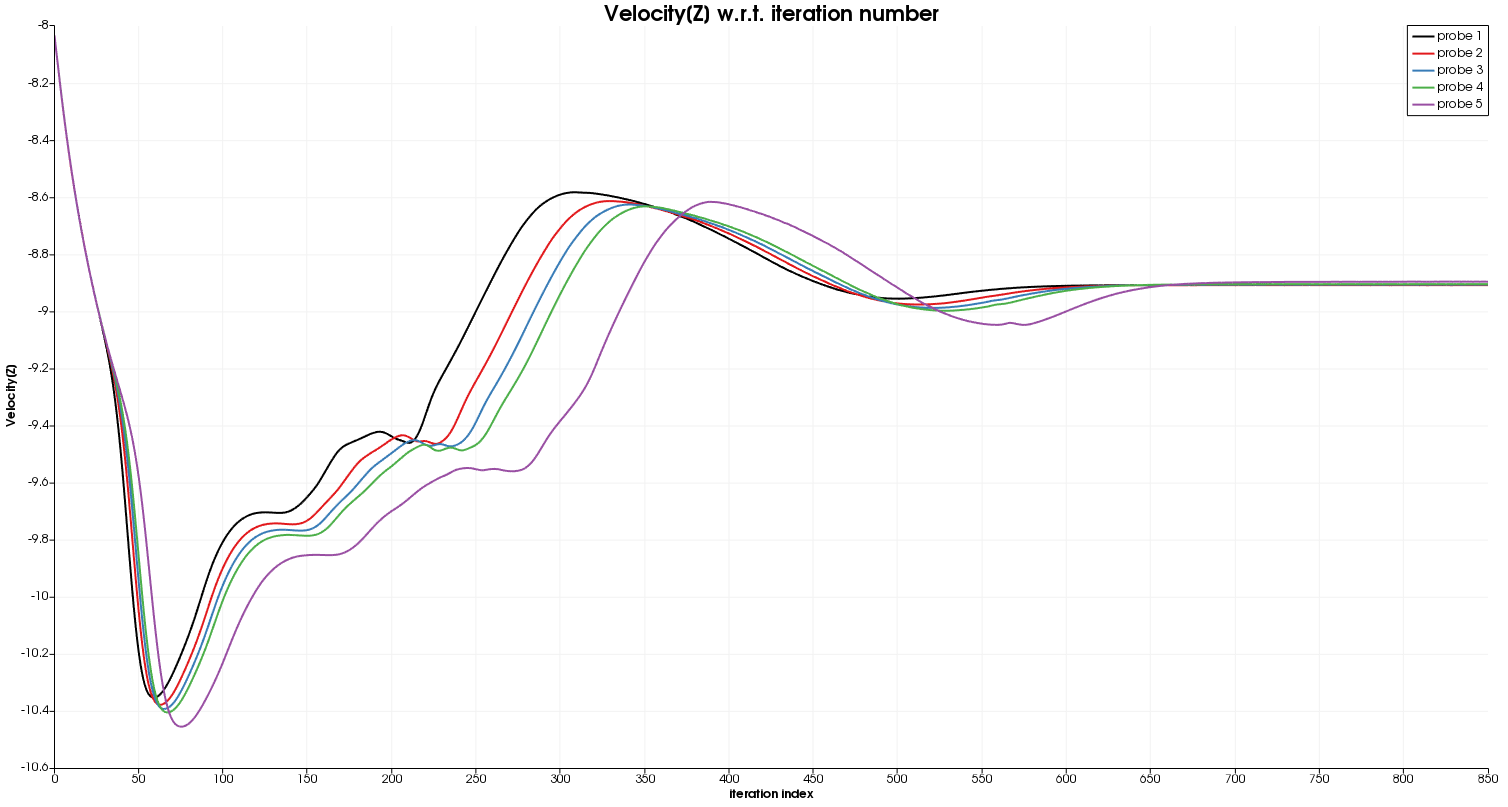
\includegraphics[width=0.8\textwidth]{\IMAGES/Part4_RANS/axial_velocity_conv.png}
\caption{Evolution of axial velocity during the calculation}
\label{lag:cap2_monit}
\end{figure}
%
\begin{figure}[H]
\centering
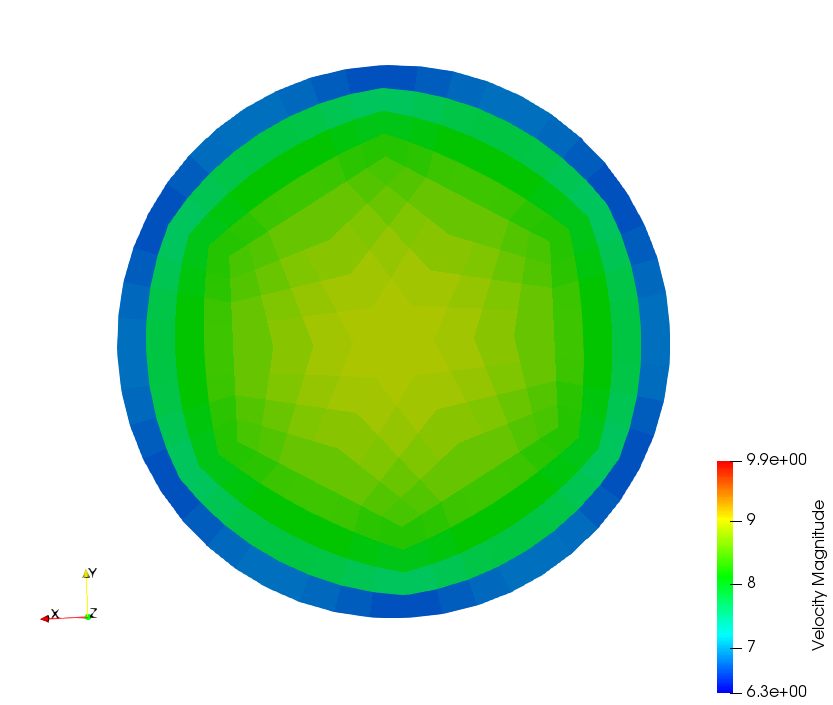
\includegraphics[width=0.5\textwidth]{\IMAGES/Part4_RANS/axial_velocity.png}
\caption{Velocity magnitude at outlet}
\label{lag:axial_velocity}
\end{figure}
%
Having generated the steady-state, single phase RANS flow field on which the particles will be injected, the first step of the one-way coupling, two phase Lagrangian \CS modelling of Arnason's \cite{Arnason} experiments has now been completed.  You can proceed to the setting-up, running, and analysis of the two phase Lagrangian \CS model.

\section{Two-Phase Lagrangian Computation}

\subsection{What you Will Learn}

In this part of the tutorial, you will learn how to set-up, run, and post-process a Lagrangian two-phase flow simulation in \CS, and how to compare the numerical results with the experimental data of \cite{Arnason}.

\subsection{Create a case with ``copy-from'' feature}

In the following, only the modifications that need to be applied to the single phase flow set-up for the Lagrangian calculation are discussed.  Everything else remains as described previously. The information added for the Lagrangian particulates include the specification of the injection point for a particle size of $5\mu m$ diameter.

In order to {\bf avoid setting again} the RANS case as described in the previous section, the second case will be created using the ``copy-from'' feature. In \salome object browser, right click on the study name ``ARNASON'' and select \keys{Add case}. Then in the pop-up window, enter the name ``RANS\_rij\_SSG\_5M'' for example, toggle the option \keys{copy from existing case} and choose the first case directory ``RANS\_rij\_SSG''. Finally click on \keys{OK}.

\subsection{Setting up the Lagrangian Simulation}

Right click on the file setup.xml in the ‘RANS\_rij\_SSG\_5M/DATA’ directory which was just created in the object browser and select \keys{Open GUI}. Check that the directory of the case is ‘RANS\_rij\_SSG\_5M and the name of the file is setup.xml (if you see unnamed instead, close the file and repeat the instruction correctly).

You can now set-up the Lagrangian two-phase flow case.

\subsubsection{Setting up the Lagrangian Model}

\paragraph{Calculation Features:}

In the panel of the 'Calculation features' section, select ‘Frozen carrier flow’ in the drop down menu of the ‘Eulerian-Lagrangian model’ menu under the ‘Additional Features’ head as shown in \figurename~\ref{lag:flow_physics}.
%
\begin{figure}[H]
\centering
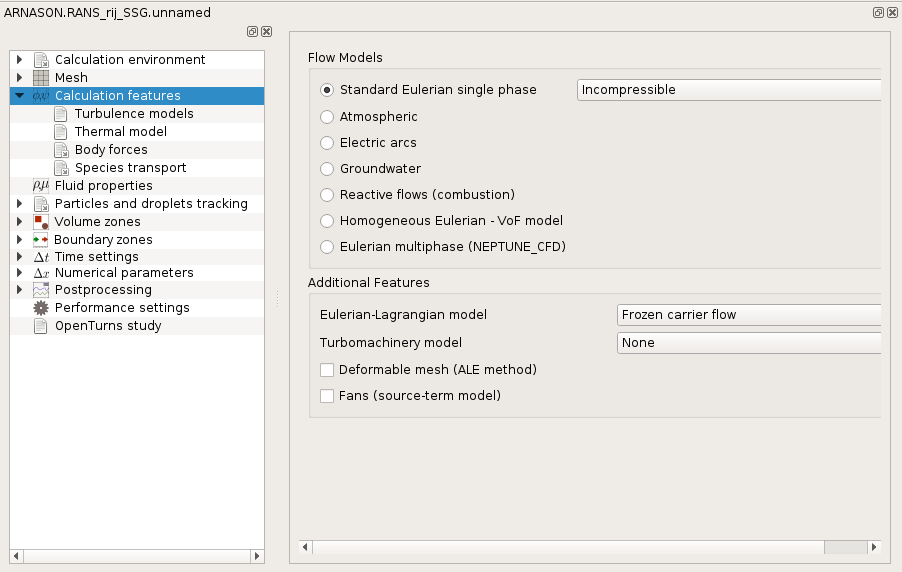
\includegraphics[width=0.8\textwidth]{\IMAGES/Part5_Lagrangian_computation/Lagr_calculation_features.png}
\caption{Selecting the flow physics.}\label{lag:flow_physics}
\end{figure}
%
\paragraph{Particles and Droplets Tracking:}

In the \menu{Particles and droplets tracking} folder that has now appeared in the GUI tree menu, click on the sub-folder \menu{Global settings} to display the panel.  By choosing 'Frozen carrier flow' in the previous section, the box ‘The continuous phase flow is a steady flow’ has been automatically ticked.  Leave all other settings in this panel at their default options.
%
\begin{figure}[H]
\centering
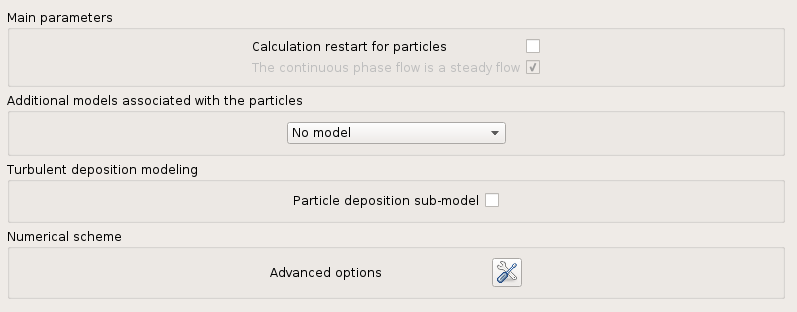
\includegraphics[width=0.8\textwidth]{\IMAGES/Part5_Lagrangian_computation/lagr_global_settings.png}
\caption{Global settings menu.}\label{lag:global_setting}
\end{figure}
%
Click on the ‘Advanced options’ icon to specify the numerical scheme, as shown in \figurename~\ref{lag:advanced_option}.  Let the other options at their default values. They should be ‘first order scheme’ for the ‘integration for the stochastic differential equations’ option and the ‘particle turbulent dispersion’ box should be ticked.
%
\begin{figure}[H]
\centering
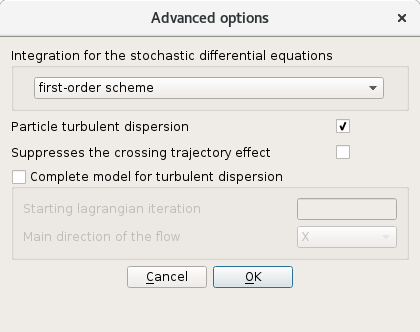
\includegraphics[width=0.6\textwidth]{\IMAGES/Part5_Lagrangian_computation/lagr_advanced_options.png}
\caption{Advanced options of the numerical scheme menu.}\label{lag:advanced_option}
\end{figure}
%
In the ‘Statistics’ sub-folder, select all parameters, as presented in \figurename~\ref{lag:statistics_menu}.  The number of particles present in the computational domain is constant after 150 iterations, hence the statistics are started after iteration 400 (cf. \figurename~\ref{lag:nb_particles} in \ref{lag:Resu_flow_field}).
%
\begin{figure}[H]
\centering
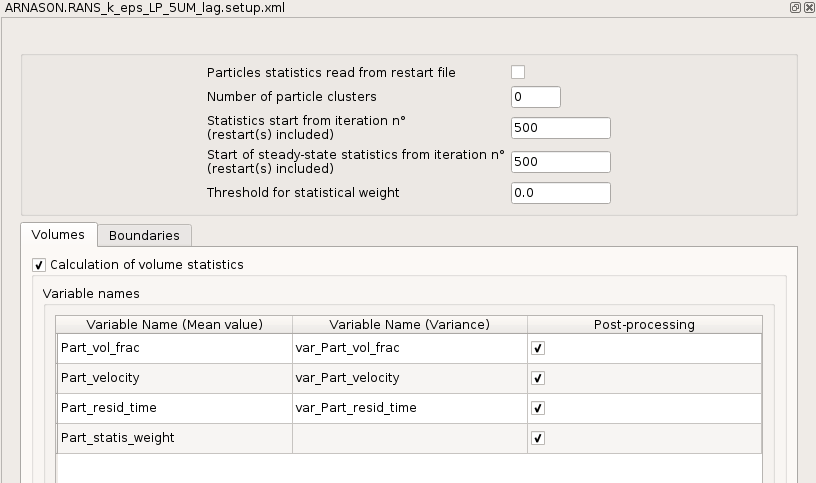
\includegraphics[width=0.8\textwidth]{\IMAGES/Part5_Lagrangian_computation/lagr_stat.png}
\caption{Statistics menu.}\label{lag:statistics_menu}
\end{figure}
%
In the panel of the \keys{Output control} sub-folder under the \keys{Postprocessing} section, ensure that the ‘Output listing at each time step’ is set to 1 for ``log frequency for particles''.  This will output particle information at every time step. In the \keys{Lagrangian solution control} subfolder, select all the options for the different variables to save.  The final set-up for this panel is shown in \figurename~\ref{lag:output_menu} and \figurename~\ref{lag:lagrangian_solution_control}.

\begin{figure}[H]
\centering
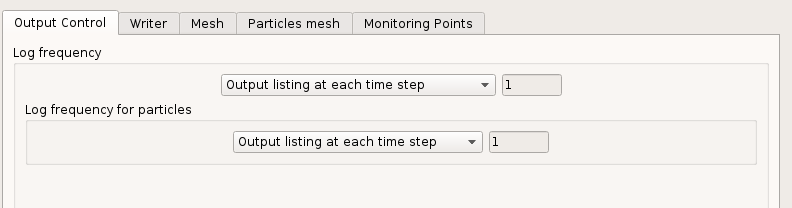
\includegraphics[width=0.8\textwidth]{\IMAGES/Part5_Lagrangian_computation/lagr_output_frequency.png}
\caption{Output menu.}\label{lag:output_menu}
\end{figure}

\begin{figure}[H]
\centering
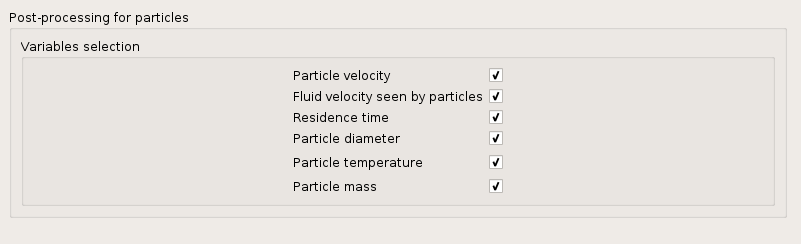
\includegraphics[width=0.8\textwidth]{\IMAGES/Part5_Lagrangian_computation/lagrangian_solution_control.png}
\caption{Solution controls.}\label{lag:lagrangian_solution_control}
\end{figure}

\paragraph{Volume zones}

In the experiments, the particles are injected further downstream of the pipe's inlet plane.  Therefore, we inject particles inside a volume section selected to contain the experiment's injection point. The injection will be defined below using the \textit{cs\_user\_lagr\_injection} and \textit{cs\_user\_lagr\_volume\_conditions} user functions but the zone has to be defined in the GUI.

In the section \menu{Volume zones > Definition of volume regions}, define a volume zone in which particles will be injected.
Name it ``particle\_injection'' and set ``injection'' in the selection criteria field to define it as shown on \figurename~\ref{lag:volume_zone_injection}.
Notice, that this zone has no ``nature'' defined for now, since its nature will be defined later in \textit{cs\_user\_lagr\_volume\_conditions}.
%
\begin{figure}[H]
\centering
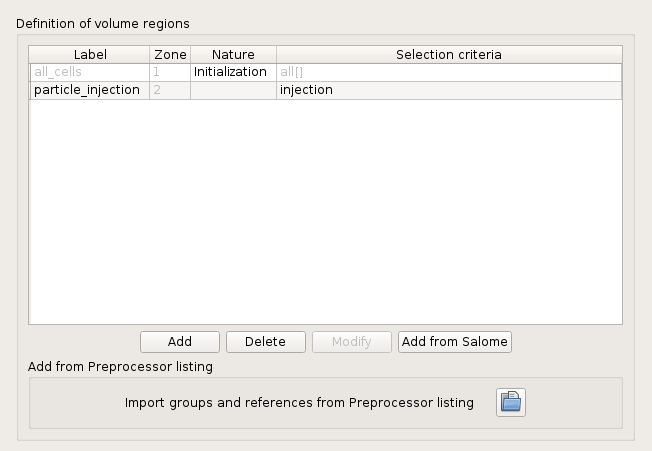
\includegraphics[width=0.8\textwidth]{\IMAGES/Part5_Lagrangian_computation/volume_zone_injection.png}
\caption{Definition of the volume zone in which particles will be injected.}\label{lag:volume_zone_injection}
\end{figure}
%

\paragraph{Particle Boundary Conditions:}

The next step is to set the ‘Particles boundary conditions’, which specify the boundary conditions for the particulate field.

Add the 'inlet' boundary in the \keys{Definition of boundary regions} sub-folder, but do not specify the boundaries further in this folder.  These will be specified for the particles in the \keys{Particles boundary conditions} sub-folder.

Go to the \keys{Particles boundary conditions} sub-folder and ensure that the type of ‘Particle-boundary interaction’ for the three boundary conditions inlet, outlet and wall are as follows:
%
\begin{itemize}
\item 'outlet': ‘Particles outlets’
\item ‘wall’: ‘Particles rebound’ $\Rightarrow$ particles bounce off walls without loss of energy
\item ‘inlet’: ‘Particles inlet’
\end{itemize}
%
This concludes the set-up of the specifics of the Lagrangian two-phase mode.  To complete the model in the GUI before moving to the required user coding, the numerical parameters should now be specified.

\subsubsection{Numerical Parameters}

In the \keys{Numerical Parameters} folder, leave all settings at the values set for the RANS calculation in the \keys{Global parameters} and \keys{Equation parameters} sub-folders.

In the \keys{Time step} panel specify a reference time step of 0.002s with 3000 iterations.  This will run the two-phase flow calculation for 2000 iterations, given that a \CS restart incudes the number of iterations previously completed.  The final set-up for this panel is shown in \figurename~\ref{lag:time_step_menu}.

\begin{figure}[H]
\centering
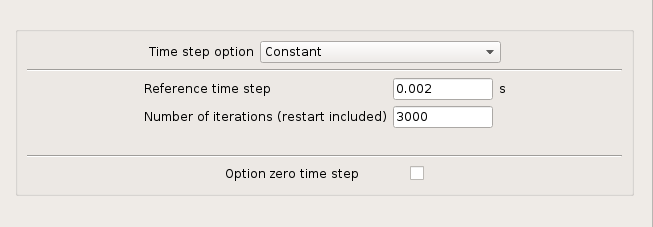
\includegraphics[width=0.8\textwidth]{\IMAGES/Part5_Lagrangian_computation/lagr_time_step.png}
\caption{Time step menu.}\label{lag:time_step_menu}
\end{figure}


\subsubsection{Start/Restart}

In the ‘Time settings’ section, go to the ‘Start/Restart’ sub-sectin to choose the restart file of the single phase fluid calculation.  Then tick the ‘Calculation on frozen velocity and pressure fields’ box as shown in \figurename~\ref{lag:start_restart_menu}, so that the particle field is injected on top of the previously calculated single-phase field.

\begin{figure}[H]
\centering
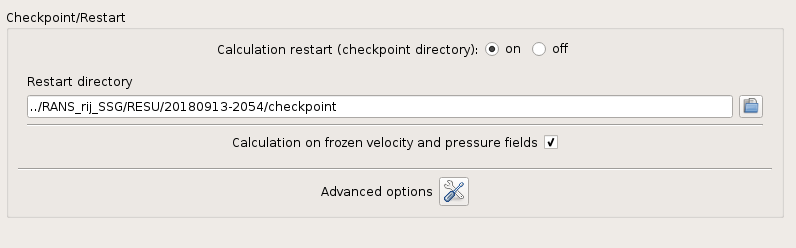
\includegraphics[width=0.8\textwidth]{\IMAGES/Part5_Lagrangian_computation/lagr_restart.png}
\caption{Start/restart menu.}\label{lag:start_restart_menu}
\end{figure}

The set-up of the two-phase flow model in the GUI is now complete.  If not already done, you should now save the 'xml' setup file.  Before you can run the simulation, user functions in \textit{cs\_user\_lagr\_particle.c}, \textit{cs\_user\_lagr\_volume\_conditions.c} and \textit{cs\_user\_postprocess.c} must be implemented in order to  define the injection in the volume and to add output statistics concerning the particles concentrations and the particle axial and radial velocities at the experimental measurement planes.

\subsection{Programming in user defined functions}\label{lag:user_coding}

Copy the sample files \textit{cs\_user\_lagr\_particle.c}, \textit{cs\_user\_lagr\_volume\_conditions.c} and \textit{cs\_user\_postprocess.c} from the tutorial directory

/../ARNASON/RANS\_rij\_SSG\_5M/SRC/REFERENCE

 to your SRC directory in order to create a local copy.  These local copies can be customised and will automatically be compiled and linked to the ‘cs\_solver’ executable at run time.

\subsubsection{\textit{cs\_user\_lagr\_volume\_conditions.c} User Functions}\label{lag:cs_user_lagr_volume_conditions.c}

Open your local version of the file using the text editor of your choice.  The specification of the injection boundary conditions for the particles is done in the \textit{cs\_user\_lagr\_volume\_conditions} function. Currently, injecting particles inside the volume is not available using the graphical interface, so programming this function is necessary.

The customised code is provided with this tutorial which can be used directly or used as a working example.  Here we describe the main parts of this code and the logic behind them.

\begin{enumerate}
\item Get the volume zone of injection defined in the GUI.
\item Define an injection set for that zone in \textit{cs\_user\_lagr\_volume\_conditions}.
\end{enumerate}

\subsubsection{\textit{cs\_user\_lagr\_particle.c} User Functions}\label{lag:cs_user_lagr_particle.c}

Open your local version of the particle tracking C file using the text editor of your choice. The aim here is to set the positions of the injected particles at each iteration on the pipe axis. The customised code is provided with this tutorial which can be used directly or used as a working example.

\subsubsection{\textit{cs\_user\_postprocess.c} User Functions} \label{lag:cs_user_postprocess.c}

The \textit{cs\_user\_postprocess\_writers}, \textit{cs\_user\_postprocess\_probes}, and \textit{cs\_user\_postprocess\_values} functions from the \textit{cs\_user\_postprocess.c} file are used to generate additional output data relating to the particles. The customised code is provided with this tutorial which can be used directly or used as a working example.  Here we describe the main parts of this code and the logic behind them:

\begin{enumerate}
\item Specify the four measurement planes where the Lagrangian statistics will be calculated
\item Give a name to the four files that will be used by the subroutine to export particle data
\item Initialise the ‘mean dispersed phase velocity’ and the ‘dispersed phase volumetric concentration’ parameters which are required to extract particle data (using the graphical interface)
\item Cycle across all cells of each measurement plane to extract the particle concentrations and the particle radial and axial velocities
\end{enumerate}

The case is now ready to run.

\subsection{Running and Analysing the Simulation}

To launch the simulation, click on the {\color{eblue} \bf Run or submit solver} button as shown below:

\begin{figure}[H] 
\centering
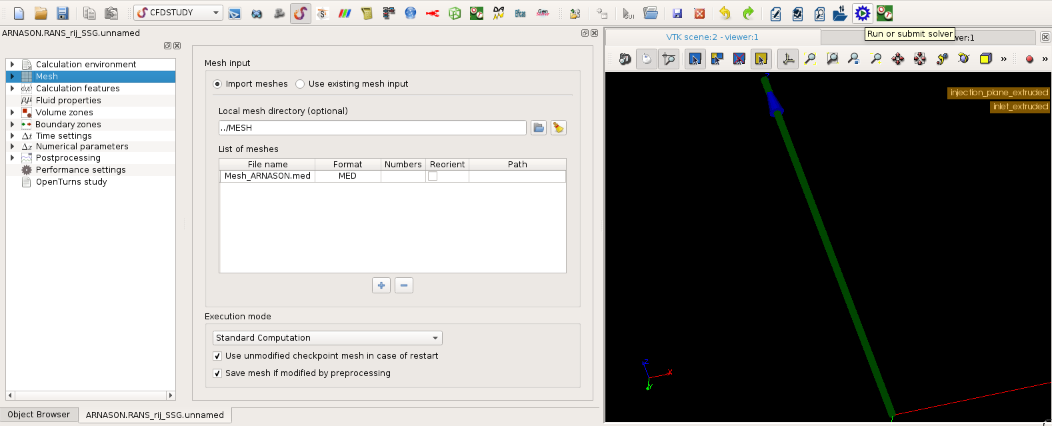
\includegraphics[width=\textwidth]{\IMAGES/Part4_RANS/run_submit_solver.png} 
\caption{Run}
\label{lag:cap1_run}
\end{figure}

A window will open where you can specify the run options.

All options except the number of processes are let to their default values:

\begin{itemize}
\item ‘runcase’ for the ‘Script file’
\item ‘1’ for the number of threads per process
\item build type to '[default]'.
\end{itemize}

Again, you may increase the ‘Number of processes’, depending on the number of cores available on your machine in order to run the simulation in parallel.

\begin{figure}[H]
\centering
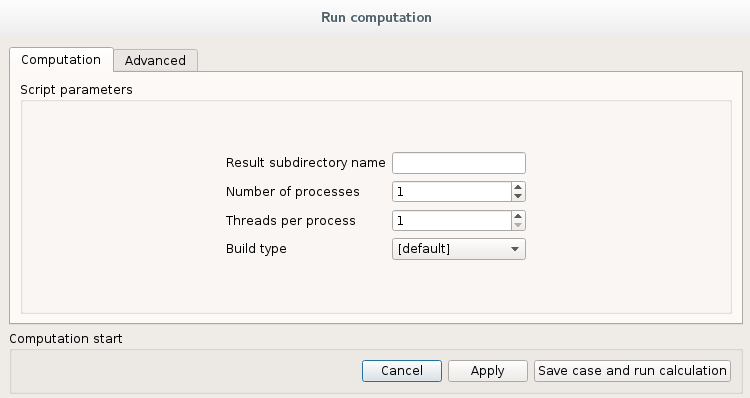
\includegraphics[width=0.7\textwidth]{\IMAGES/Part5_Lagrangian_computation/lagr_nb_proc.png}
\caption{Batch calculation settings.}\label{lag:batch_calculation_setting}
\end{figure}

Press the ‘Save case and run calculation’ button to run \CS.  The pop-up panel for the run opens, listing in real time the different stages of the calculation, from compilation of the user-subroutines to the saving of the results.

\subsection{Post-processing the Results}

For the post-processing of the results, move to the \paravis module.  In the ‘Pipeline Browser’ panel on the left-hand side, right click and select \keys{Open} in the drop-down menu.  Point to the ‘RESULTS.case’ file in the RESU directory for the run that has just finished:

'/../ARNASON/RANS\_rij\_SSG\_5M/RESU/DateOfRunTimeOfRun/postprocessing/RESULTS\\.case'

and to the 'PARTICLES.case' in:

'/../ARNASON/RANS\_rij\_SSG\_5M/RESU/DateOfRunTimeOfRun/postprocessing\\/PARTICLES.case.'

Follow the steps described in tutorials \cite{ShearDriven_Tuto, HeatedDriven_Tuto}, to create the ‘ExtractBlock’ and ‘CellDataPointData’ objects, and post-process the results.



\section{Results analysis}

\subsection{What you Will Learn}

In this final part of the tutorial, you will learn how to analyse in detail the calculated particle field and compare it to the single-phase field, and to compare the numerical and experimental results using the particle output file that you set-up in the \textit{cs\_user\_postprocess.c} user functions.

\subsection{Verifying the Simulation}\label{lag:verify}

During the Lagrangian calculation, a ‘listla’ file is automatically created by \CS containing the data listed in \tablename~\ref{lag:listla}:

\begin{table}[H]
\begin{center}
\begin{tabular}{c l}
\Mline
\bf \ \ \ \ \ Column \ \ \ \ \  & \bf Description  \\
\hline\hline
1 & Number of the time step  \\
2 & Lagrangian physical time \\
3 & The number of instantaneous particles in the domain \\
4 & The number of instantaneous particles in the domain (with weighting) \\
5 & The number of particles injected in the domain \\
6 & The number of particles injected in the domain (with weight) \\
\multirow{2}{*}{7} & Instantaneous number of particles leaving the domain, \\
 & or deposed and eliminated \\
\multirow{2}{*}{8} & Instantaneous number of particles leaving the domain, \\
 & sticking to the wall and eliminated(with weighting) \\
9 & Instantaneous number of particles sticking to the wall \\
10 & Instantaneous number of particles sticking to walls (with weighting) \\
11 & Instantaneous number of particles lost \\
\Mline
\end{tabular}
\caption{Description of the data in the ‘listla’ file..\label{lag:listla}}
\end{center}
\end{table}

This information can be used to evaluate the convergence of the simulations.

For example, \figurename~\ref{lag:nb_particles} and \figurename~\ref{lag:particles_leaving} present, respectively, the number of particles in the domain and the number of particles entering and leaving the domain during the Lagrangian simulation.  It can be seen that both the number of particles in the domain and the number of particles leaving the domain is well established and remains stable after less than 200 time steps. The earlier decision, when setting up the Lagrangian model, of starting the particle statistical analysis at the $500^{th}$ time step is validated by this analysis.
%
\begin{figure}[H]
\centering
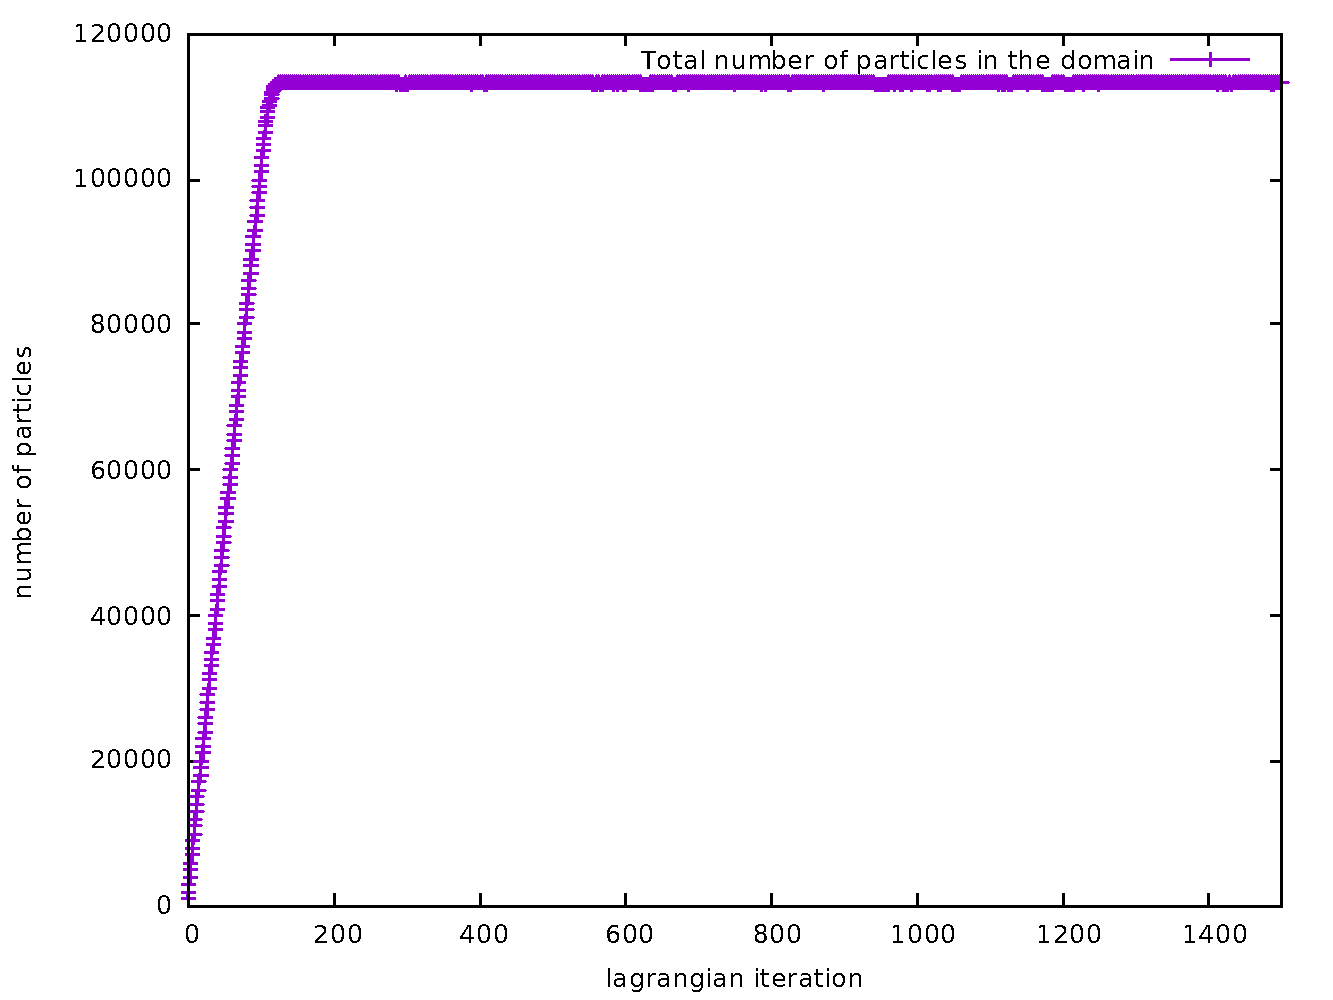
\includegraphics[width=0.7\textwidth]{\IMAGES/Part6_Results/particles_domain.pdf}
\caption{Number of particles in the computational domain over the first 1500 lagrangian iterations.}\label{lag:nb_particles}
\end{figure}
%
\begin{figure}[H]
\centering
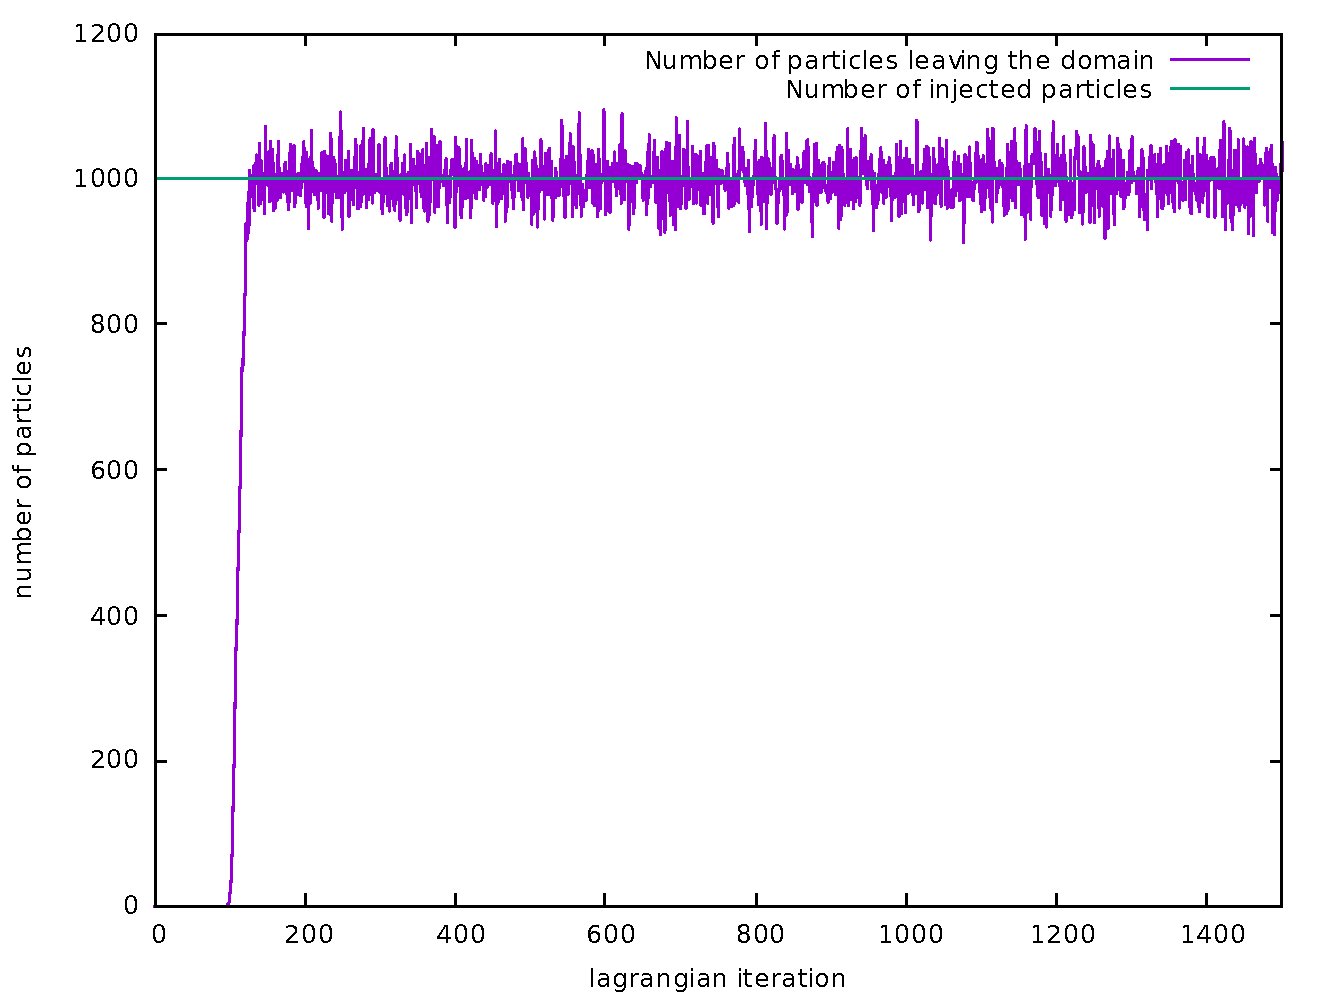
\includegraphics[width=0.7\textwidth]{\IMAGES/Part6_Results/particles_in_out.pdf}
\caption{Number of particles entering and leaving the computational domain over the first 1500 lagrangian iterations.}\label{lag:particles_leaving}
\end{figure}
%
\subsection{Flow Field}\label{lag:Resu_flow_field}

Starting with the analysis of the flow field in \paravis, \figurename~\ref{lag:part_vol_frac} presents a countour plot of the particle volume fraction in a 2D plane along the centre line of the pipe.  It can be seen that the majority of the particles injected into the flow domain remain along or near the pipe axis before spreading in spanwise direction.
%
\begin{figure}[H]
\centering
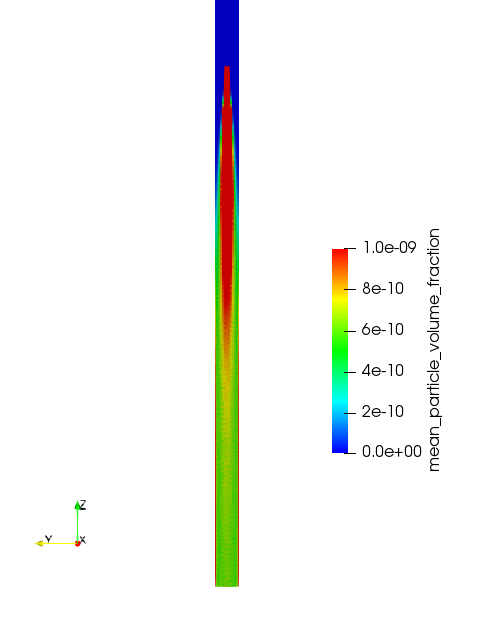
\includegraphics[width=0.8\textwidth]{\IMAGES/Part6_Results/lagr_part_vol_frac_crop.png}
\caption{Volume fraction of the particles in the pipe.}\label{lag:part_vol_frac}
\end{figure}
%
\figurename~\ref{lag:v_z} presents the $V_z$ velocity component of the carrier fluid, the vertical velocity of the particles and the $V_z$ velocity variance of these particles, also on 2D slices in the yz plane along the pipe centre line.
%
\begin{figure}[H]
\begin{subfigure}{0.3\textwidth}
\centering
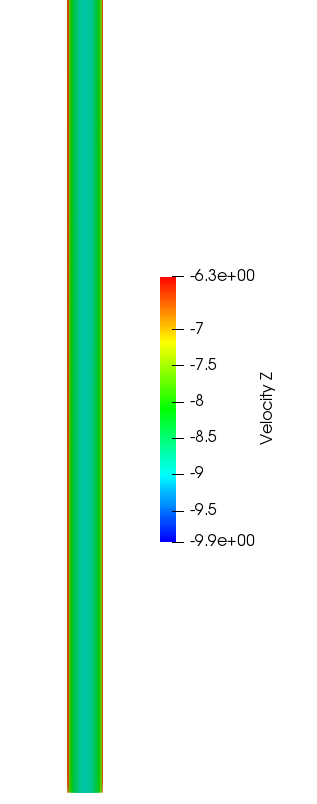
\includegraphics[width=\textwidth]{\IMAGES/Part6_Results/lagr_vel_z_crop.png}
\caption{$V_z$ velocity of the fluid\\ \ \ }
\label{lag:cap1_vel}
\end{subfigure}
\begin{subfigure}{0.3\textwidth}
\centering
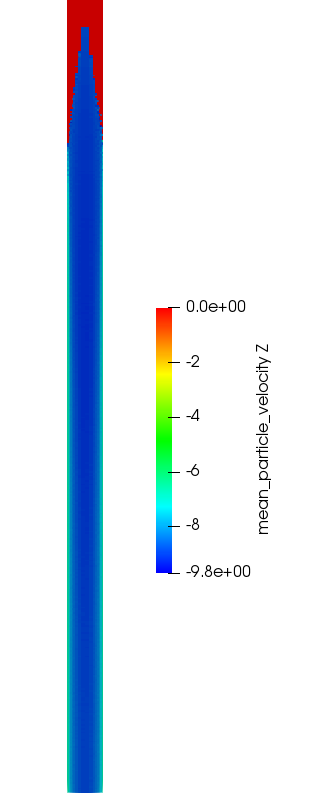
\includegraphics[width=\textwidth]{\IMAGES/Part6_Results/lagr_part_vel_z_crop.png}
\caption{$V_z$ velocity of the particles\\ \ \ }
\label{lag:cap2_vel}
\end{subfigure}
\begin{subfigure}{0.3\textwidth}
\centering
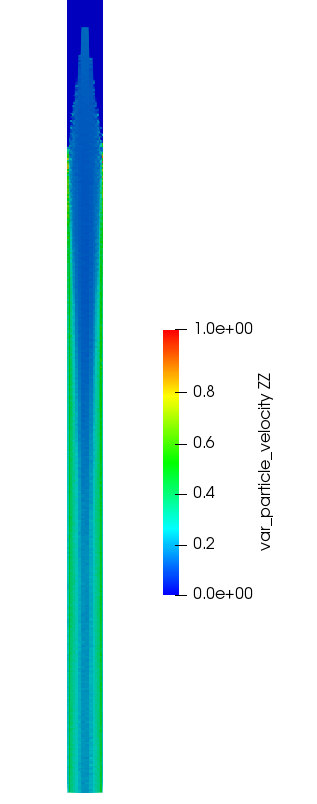
\includegraphics[width=\textwidth]{\IMAGES/Part6_Results/lagr_var_part_vel_z_crop.png}
\caption{Variance of the $V_z$ velocity of the particles}
\label{lag:cap3_vel}
\end{subfigure}
\caption{Visualization in the yz plane along the pipe axis}
\label{lag:v_z}
\end{figure}
%
It can be seen that, as the particles are very small, they are entrained by the fluid at the fluid velocity, with both the carrier fluid and the particles achieving a maximum velocity of the order of -9.5m/s, \figurename~\ref{lag:cap1_vel} and \figurename~\ref{lag:cap2_vel}.

The particle response and flow time scales may be compared to verify that, in this instance, the particles are expected to closely follow the carrier fluid.   For this low particle-Reynolds number flow, the relaxation time, $\tau_p$, of the particle is given by:

\begin{equation}
\tau _p \approx \dfrac{\rho_pd_p^2}{18\mu}=1.92\times10^{-4}s
\end{equation}

For turbulent dispersion, the flow time scale may be estimated as the characteristic time of the turbulence,$\tau^t_{12}$, calculated at the injection point:

\begin{equation}
\tau^t_{12}=\dfrac{3}{2}C_\mu\dfrac{k^2}{\epsilon}=2.726\times10^{-3}s
\end{equation}

Therefore,$\frac{\tau_p}{\tau^t_{12}}\ll1.0$, which confirms that the particles will follow the carrier fluid turbulence.

The variance of the vertical velocity of the particles (\figurename~\ref{lag:cap3_vel}) can be seen to be at a minimum along the pipe axis and at its highest close to the flow domain wall, due to the near wall effects such as the boundary layer and the particle rebound condition.

\subsection{Comparison of Predicted and Experimental Data}

The numerical and experimental data can be compared using the output data files 'Z318.csv', 'Z502.csv', 'Z679.csv', 'Z132.csv' which \CS wrote at the end of the calculation as a result of the programming in \textit{cs\_user\_postprocess.c} (\ref{lag:cs_user_postprocess.c}).

These files contain the particle normalised axial velocity, the particle concentration and the particle radial velocity at the $z = 0,318$, $z = 0,502$, $z = 0,679$ and $z = 1,32m$ planes where experimental data is also available. For convenience, the experimental data at these locations has been reproduced in Appendix \ref{lag:appendixA} from \cite{Arnason}.

\figurename~\ref{lag:z0318} to \figurename~\ref{lag:z132} present the predicted (green line) and measured (red symbols) data at the different measuring planes. The figures show that the calculated values of the axial velocity and  particle concentration are in rather good agreement with the experimental data for all measurement planes.  The radial component of the velocity is also in good agreement with the experiment data, except for z = 1.32m.  As the radial velocity decreases with the distance from the injection point and the concentration of particles near the walls increases, the error in the numerical results increases.

\begin{figure}[H]
\begin{subfigure}{0.33\textwidth}
\centering
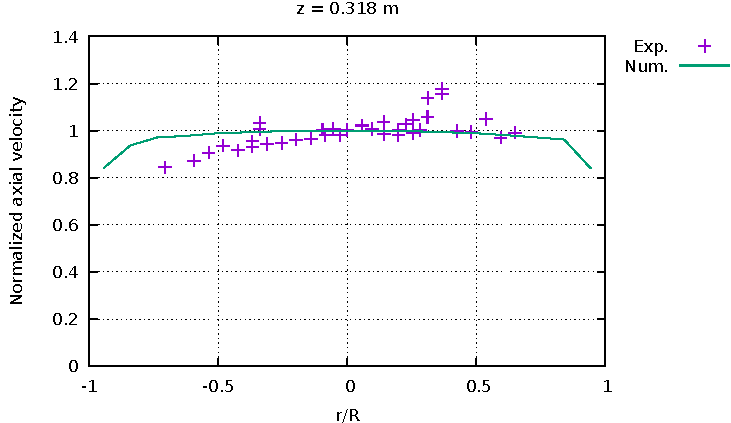
\includegraphics[width=\textwidth]{\IMAGES/Part6_Results/axial_z0318.pdf}
\caption{Axial velocity}\label{lag:axial_z0318}
\end{subfigure}
\begin{subfigure}{0.33\textwidth}
\centering
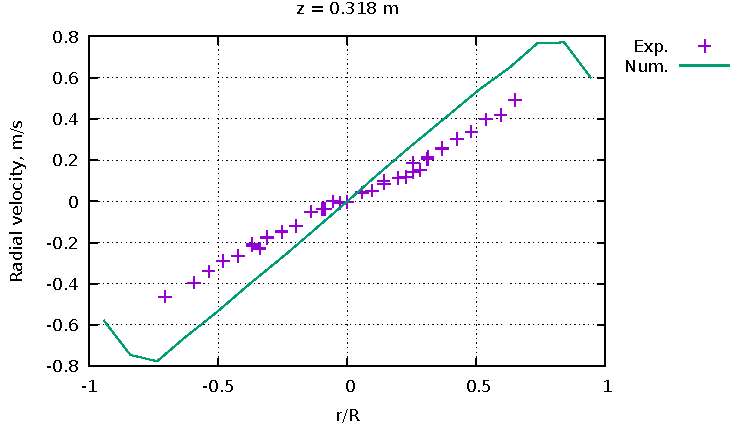
\includegraphics[width=\textwidth]{\IMAGES/Part6_Results/radial_z0318.pdf}
\caption{Radial velocity}\label{lag:radial_z0318}
\end{subfigure}
\begin{subfigure}{0.33\textwidth}
\centering
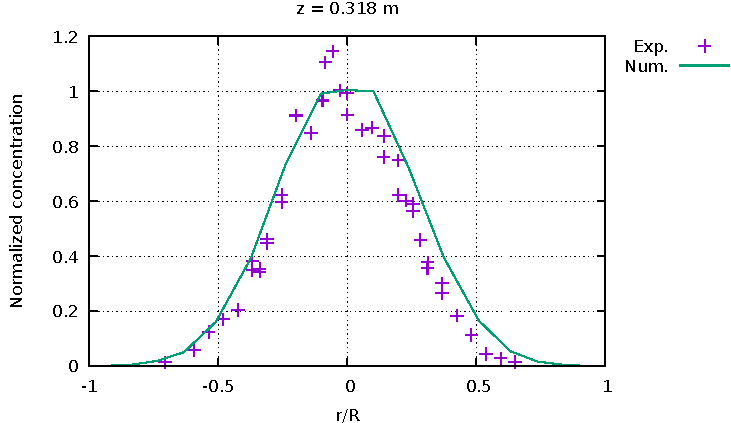
\includegraphics[width=\textwidth]{\IMAGES/Part6_Results/concentration_z0318.pdf}
\caption{Particle concentration}\label{lag:conc_z0318}
\end{subfigure}
\captionsetup{justification=centering}
\caption{Numerical (line) and experimental\cite{Arnason} (symbols) results at z = 0.318m.}
\label{lag:z0318}
\end{figure}

\begin{figure}[H]
\begin{subfigure}{0.33\textwidth}
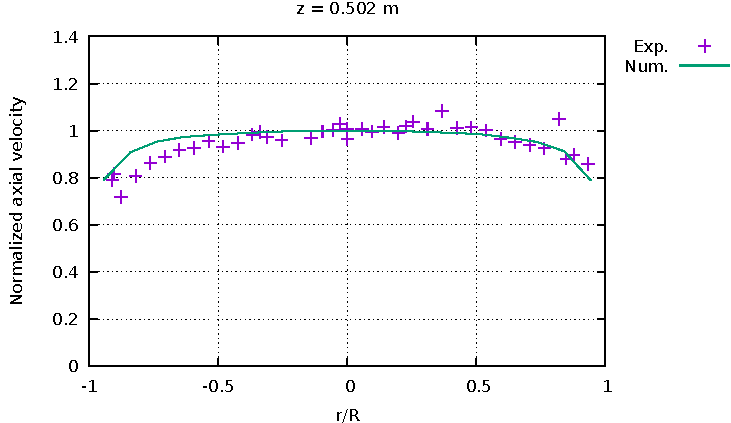
\includegraphics[width=\textwidth]{\IMAGES/Part6_Results/axial_z0502.pdf}
\caption{Axial velocity.}\label{lag:axial_z0502}
\end{subfigure}
\begin{subfigure}{0.33\textwidth}
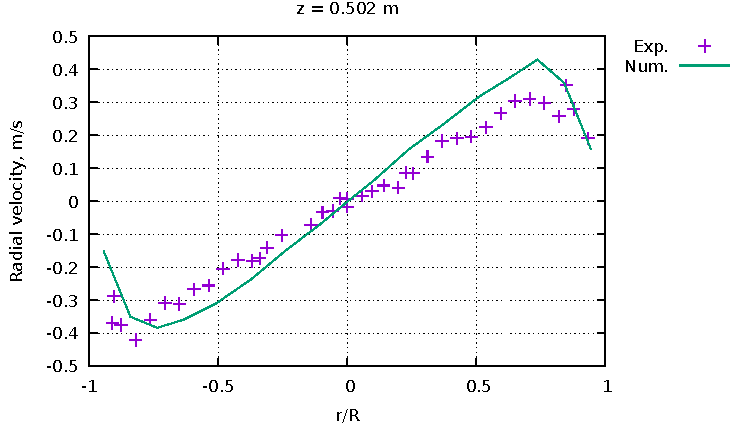
\includegraphics[width=\textwidth]{\IMAGES/Part6_Results/radial_z0502.pdf}
\caption{Radial velocity.}\label{lag:radial_z0502}
\end{subfigure}
\begin{subfigure}{0.33\textwidth}
\centering
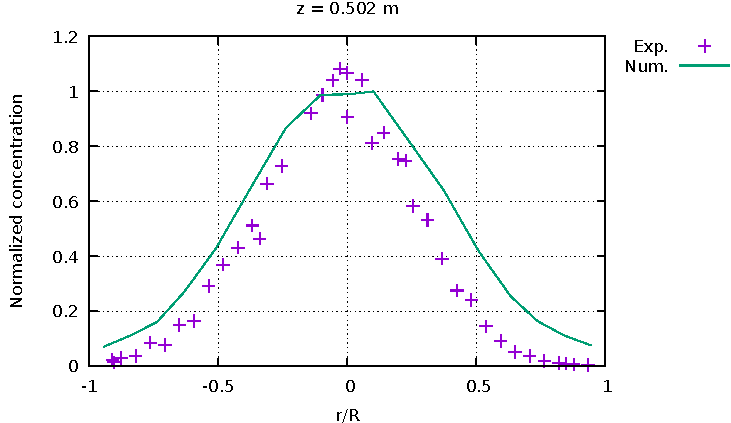
\includegraphics[width=\textwidth]{\IMAGES/Part6_Results/concentration_z0502.pdf}
\caption{Particle concentration}\label{lag:conc_z0502}
\end{subfigure}
\captionsetup{justification=centering}
\caption{Numerical (line) and experimental\cite{Arnason} (symbols) results at z = 0.502m.}
\label{lag:z0502}
\end{figure}

\begin{figure}[H]
\begin{subfigure}{0.33\textwidth}
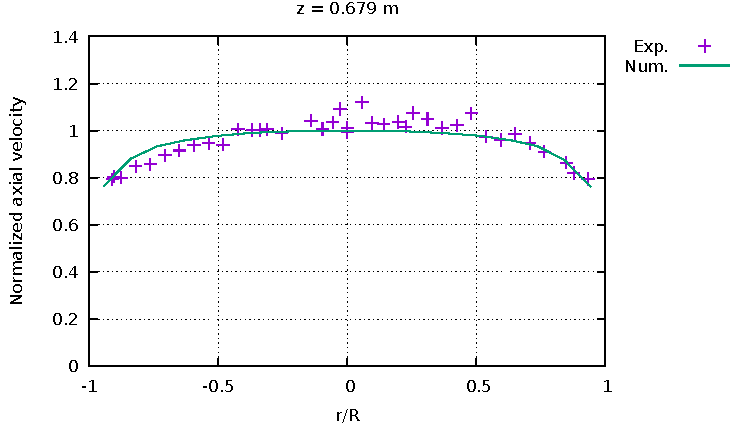
\includegraphics[width=\textwidth]{\IMAGES/Part6_Results/axial_z0679.pdf}
\caption{Axial velocity.}\label{lag:axial_z0679}
\end{subfigure}
\begin{subfigure}{0.33\textwidth}
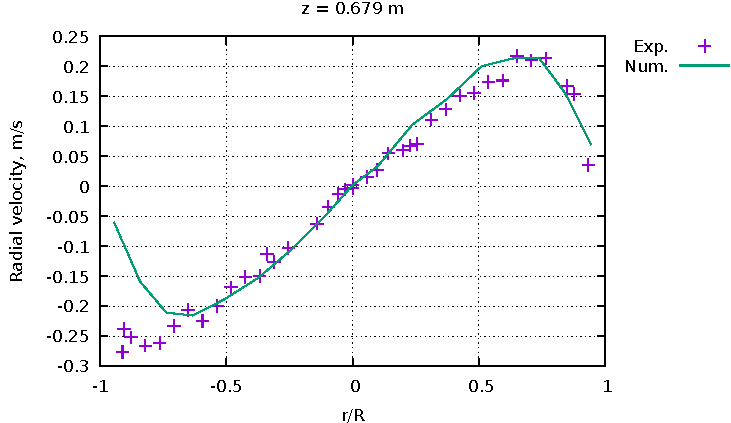
\includegraphics[width=\textwidth]{\IMAGES/Part6_Results/radial_z0679.pdf}
\caption{Radial velocity.}\label{lag:radial_z0679}
\end{subfigure}
\begin{subfigure}{0.33\textwidth}
\centering
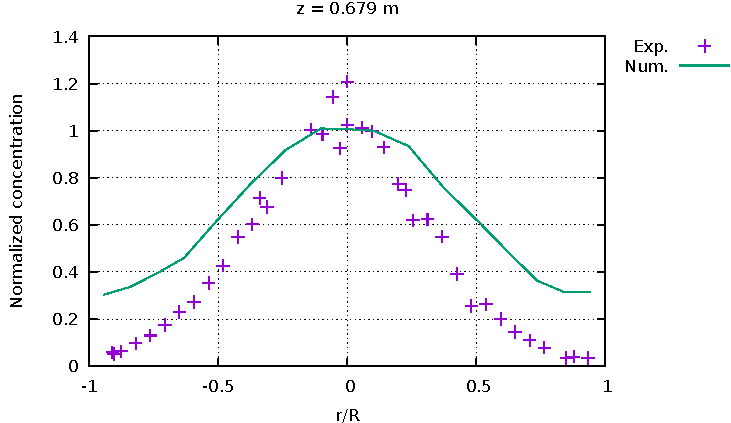
\includegraphics[width=\textwidth]{\IMAGES/Part6_Results/concentration_z0679.pdf}
\caption{Particle concentration}\label{lag:conc_z0679}
\end{subfigure}
\captionsetup{justification=centering}
\caption{Numerical (line) and experimental\cite{Arnason} (symbols) results at z = 0.679m.}
\label{lag:z0679}
\end{figure}

\begin{figure}[H]
\begin{subfigure}{0.33\textwidth}
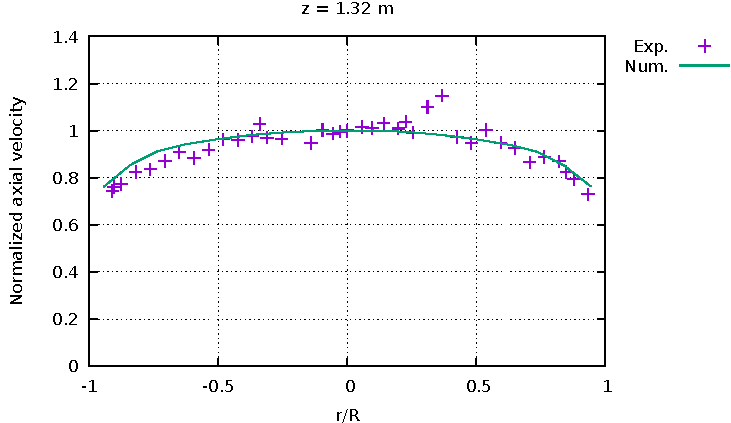
\includegraphics[width=\textwidth]{\IMAGES/Part6_Results/axial_z132.pdf}
\caption{Axial velocity.}\label{lag:axial_z132}
\end{subfigure}
\begin{subfigure}{0.33\textwidth}
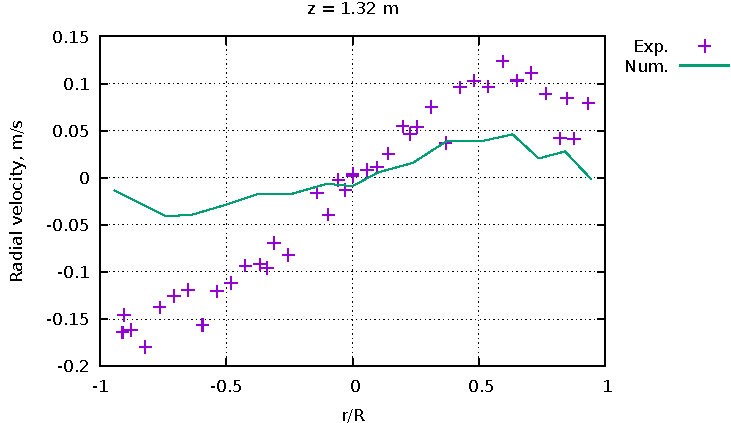
\includegraphics[width=\textwidth]{\IMAGES/Part6_Results/radial_z132.pdf}
\caption{Radial velocity.}\label{lag:radial_z132}
\end{subfigure}
\begin{subfigure}{0.33\textwidth}
\centering
\includegraphics[width=\textwidth]{\IMAGES/Part6_Results/concentration_z132.pdf}
\caption{Particle concentration}\label{lag:conc_z132}
\end{subfigure}
\captionsetup{justification=centering}
\caption{Numerical (line) and experimental\cite{Arnason} (symbols) results at z = 1.32m.}
\label{lag:z132}
\end{figure}

%\chapter{References}
\section{References}

\begin{thebibliography}{20}

\bibitem{Salome} \textcolor{blue}{\underline{\url{www.salome-platform.org}}}

\bibitem{CS_Paper}{\sc F. Archambeau, N. Méchitoua, M. Sakiz},\\
{\em \CS: a Finite Volume Code for the Computation of Turbulent
Incompressible Flows - Industrial Applications},\\
International Journal on Finite
Volumes, Vol. 1, 2004.

\bibitem{CS_Web} \textcolor{blue}{\underline{\url{www.code-saturne.org}}}

\bibitem{Arnason} {\sc G. Arnason,}\\
{\em Measurement of particle dispersion in turbulent pipe flow},\\
Washington State University, Department of Mechanical Engineering, 1982

\bibitem{ShearDriven_Tuto} {\sc EDF},\\
{\em Tutorial 1: Shear Driven Cavity Flow},\\
\CS Tutorial Series

\bibitem{hexa} \textcolor{blue}{\underline{\url{http://docs.salome-platform.org/salome_6_6_0/gui/HEXABLOCK/index.html}}}

\bibitem{HeatedDriven_Tuto} {\sc EDF},\\
{\em Tutorial 3: Heated Square Cavity Flow},\\
\CS Tutorial Series

\end{thebibliography}

\appendix
\section{Appendix A $–$ Experimental Data from \cite{Arnason}}\label{lag:appendixA}

The experimental data from ARNASON \cite{Arnason}, for the particles of $5\mu m$ diameter are presented in this appendix.  Experimental data of particle radial velocity, concentration and normalized axial velocity for the normalised radius at z = 0.318, 0.502, 0.679 and 1.32m are listed in the \tablename~\ref{lag:appendix1} to \ref{lag:appendix4} respectively.

\begin{table}[H]
\centering
\includegraphics[width=14cm]{\IMAGES/Appendix/appendix1.png}
\caption{Experimental data from ARNASON obtained for particles of $5\mu m$ \cite{Arnason} at $z=0,318$m.}\label{lag:appendix1}
\end{table}


\begin{table}[H]
\centering
\includegraphics[width=14cm]{\IMAGES/Appendix/appendix2.png}
\caption{Experimental data from ARNASON obtained for particles of $5\mu m$ \cite{Arnason} at $z=0,502$m.}\label{lag:appendix2}
\end{table}


\begin{table}[H]
\centering
\includegraphics[width=14cm]{\IMAGES/Appendix/appendix3.png}
\caption{Experimental data from ARNASON obtained for particles of $5\mu m$ \cite{Arnason} at $z=0,679$m.}\label{lag:appendix3}
\end{table}


\begin{table}[H]
\centering
\includegraphics[width=14cm]{\IMAGES/Appendix/appendix4.png}
\caption{Experimental data from ARNASON obtained for particles of $5\mu m$ \cite{Arnason} at $z=1,32$m.}\label{lag:appendix4}
\end{table}








\end{document}

